\chapter{Results}

This chapter presents a comprehensive evaluation of Neuro-\gls{SAM} and its constituent foundation model variants across the tasks of path tracing, dendrite segmentation, and dendritic spine segmentation. Building upon the modular architecture described in the Feature Work chapter, our goal is to empirically validate the performance improvements introduced by integrating foundation models into the segmentation pipeline. All models were benchmarked against \gls{DeepD3} \cite{Fernholz_2024}, which serves as the baseline due to its strong community adoption, open accessibility, and multi-rater validation framework. Through quantitative comparisons on the benchmark dataset and qualitative analysis across diverse imaging conditions, we demonstrate the strengths and limitations of each model configuration, culminating in a robust evaluation of the proposed Neuro-\gls{SAM} framework.

\section{Evaluation Protocol}
To rigorously evaluate the performance of Neuro-\gls{SAM}, we established a unified benchmarking pipeline incorporating diverse microscopy datasets, standardized metrics, and consistent evaluation logic across all models and tasks. This section outlines the datasets used, the metrics computed, and the procedures adopted for testing Neuro-\gls{SAM}.

\subsection{Datasets}
All experiments were conducted on high-resolution 3D microscopy volumes, primarily centered around the \textit{benchmark dataset} \cite{Fernholz_2024}, which offers multi-rater annotations for both dendrites and dendritic spines. Additional experiments included curated datasets with varied voxel resolutions, imaging modalities, and fluorescent indicators to test generalizability.

\subsection{Evaluation Metrics}
Segmentation quality was assessed using pixel-wise and object-level metrics, computed separately for dendrites and spines:
\begin{itemize}
\item \textbf{Intersection-over-Union}: Quantifies the overlap between predicted and ground truth masks. The \gls{IoU} can be formulated as :

\[
IoU = \frac{|P \cap G|}{|P \cup G|}
\]

where $P$ and $G$ denote the sets of predicted and ground truth foreground pixels, respectively.
\item \textbf{Dice Score}: Measures segmentation similarity, balancing precision and recall. Meanwhile the Dice Score can be computed as:

\[
Dice = \frac{2 |P \cap G|}{|P| + |G|}
\]

\item \textbf{Recall}: Fraction of ground truth instances detected by the model.
\item \textbf{Precision}: Fraction of predicted instances that correspond to true positives.
\end{itemize}

All metrics were computed on the maximum intensity projection of the dataset. In the following section, we first revisit the baseline performance of \gls{DeepD3} to contextualize the comparative evaluation.

\section{Baseline: DeepD3 Performance Overview}
To establish a consistent baseline for evaluating the segmentation performance of Neuro-\gls{SAM}, we re-ran the official \texttt{\gls{DeepD3}\_32F} model on the benchmark dataset \cite{Fernholz_2024}. \autoref{fig:deepd3_max_proj} shows a maximum intensity projection of the 3D input stack (top), along with \gls{DeepD3}'s predicted dendrite (middle) and spine (bottom) masks. As visualized, the dendrites are largely continuous and well-defined, while the spine predictions densely follow dendritic shafts, capturing a wide variety of spine shapes and sizes. However, occasional over-segmentation and background noise are also evident, particularly in regions with weak signal or closely packed structures.



\begin{center}
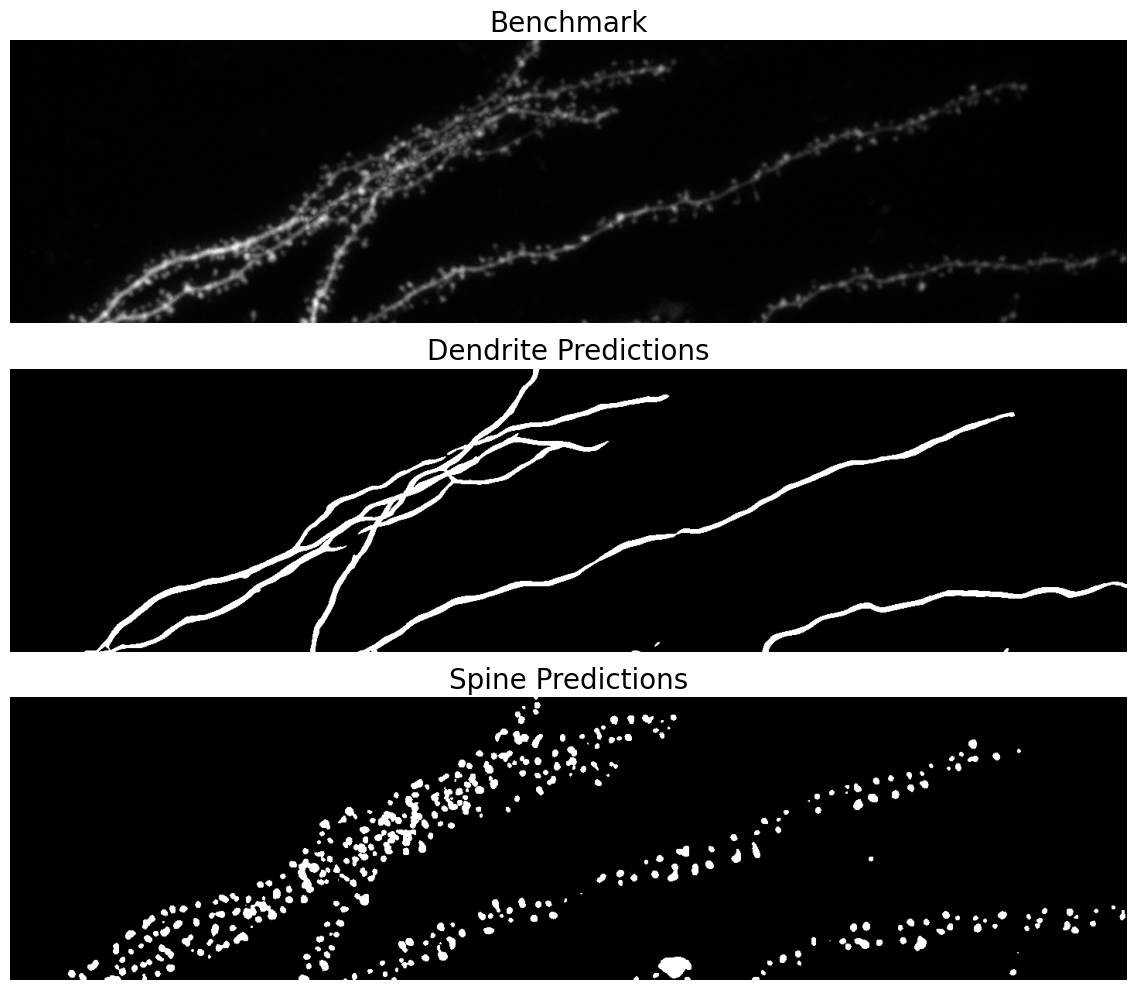
\includegraphics[width=0.7\textwidth]{figures/20_deepd3_max.png}
\captionof{figure}{\gls{DeepD3} prediction masks on the benchmark dataset. Top: Maximum intensity projection of the raw 3D microscopy stack. Middle: Dendrite prediction mask generated by the \gls{DeepD3}\_32F model. Bottom: Spine prediction mask from the same model. Scale: $0.94\,\mu\text{m}/\text{px}$}
\label{fig:deepd3_max_proj}
\end{center}

To quantify \gls{DeepD3}’s performance, predictions were compared against three expert raters (U, V, W), as well as their intersection and union masks. The full evaluation metrics Dice, \gls{IoU}, Precision, and Recall are summarized in \autoref{tab:deepd3_metrics}, with corresponding visualizations shown in \autoref{fig:deepd3_dice_iou} and \autoref{fig:deepd3_prec_recall}. For dendrites, the Dice scores range from 0.741 to 0.824 across individual raters, and 0.723 and 0.820 for the intersection and union masks, respectively. The corresponding \gls{IoU} values range from 0.416 to 0.609. In spine segmentation, \gls{DeepD3} achieves Dice scores as high as 0.775 (intersection) and 0.757 (rater W), but performance degrades when evaluated against union masks, where the \gls{IoU} drops to 0.545. This reflects the model's high specificity but occasional miss of borderline spines. 


\begin{table}[caption={Dice, \gls{IoU}, Precision, and Recall scores for dendrites and spines across raters, intersection, and union of \gls{DeepD3}.}, label=tab:deepd3_metrics]
\centering
\scriptsize
    \begin{tabular}{c c c c c c c}
        \toprule
        {\bf Rater / Consensus} & {\bf Dice Dendrites} & {\bf \gls{IoU} Dendrites} & {\bf Dice Spines} & {\bf \gls{IoU} Spines} & {\bf Precision Spines} & {\bf Recall Spines} \\ \midrule
            U & 0.815 & 0.688 & 0.587 & 0.416 & 0.632 & 0.899 \\
            V & 0.824 & 0.701 & 0.594 & 0.423 & 0.573 & 0.916 \\
            W & 0.741 & 0.589 & 0.757 & 0.609 & 0.738 & 0.850 \\
            Intersection & 0.723 & 0.775 & 0.633 & 0.519 & 0.735 & 0.850 \\
            Union & 0.820 & 0.472 & 0.545 & 0.375 & 0.455 & 0.869 \\
        \midrule
    \end{tabular}
\end{table}

\begin{center}
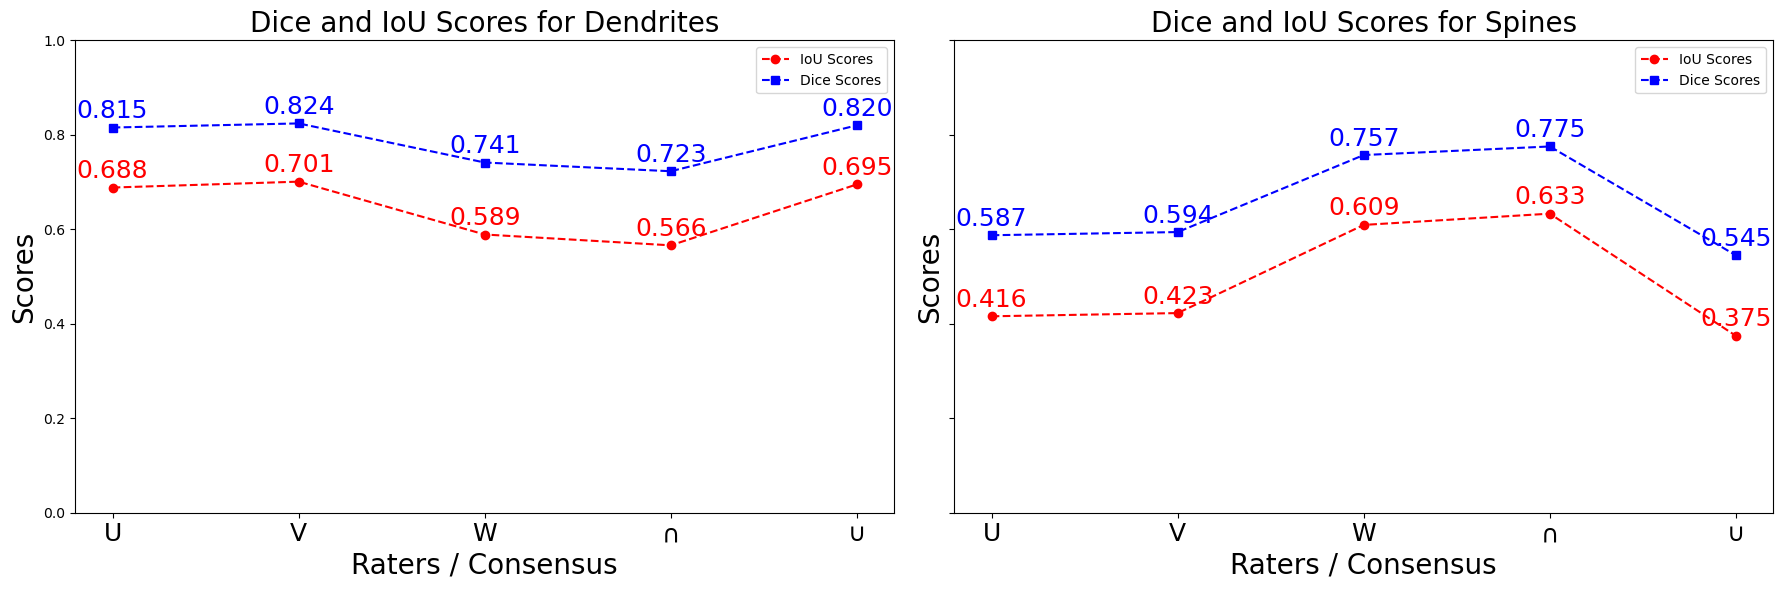
\includegraphics[width=0.95\textwidth]{figures/21_deepd3_dice_iou.png}
\captionof{figure}{Quantitative performance of \gls{DeepD3} against individual raters and consensus masks. Left: Dice and \gls{IoU} scores for dendrite segmentation across raters U, V, W, as well as intersection and union masks. Right: Dice and \gls{IoU} scores for spine segmentation using the same evaluation setup. Scale: $0.94\,\mu\text{m}/\text{px}$}
\label{fig:deepd3_dice_iou}
\end{center}

Precision and recall values further highlight the model’s detection tendencies. As shown in \autoref{fig:deepd3_prec_recall}, recall remains consistently high across all raters, peaking at 0.916 (rater V) and staying above 0.85 in all cases. Precision, however, varies more substantially, dropping to 0.455 against the union mask indicating that while the model successfully captures the majority of annotated spines, it also predicts additional structures not present in the ground truth.

\begin{center}
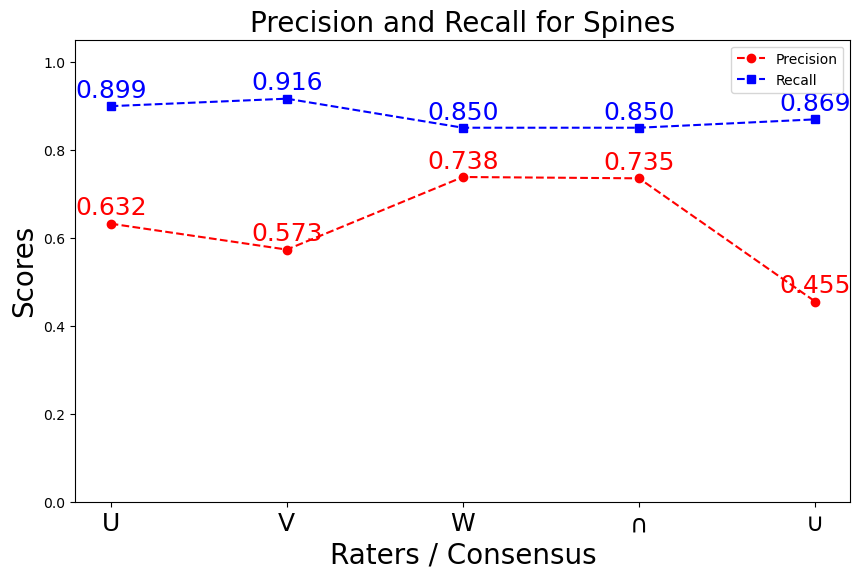
\includegraphics[width=0.7\textwidth]{figures/22_deepd3_prec_recall.png}
\captionof{figure}{Precision and recall of \gls{DeepD3} spine predictions. Recall remains consistently high across all raters and consensus masks, while precision varies more substantially, especially when evaluated against the union mask.}
\label{fig:deepd3_prec_recall}
\end{center}

A qualitative comparison between \gls{DeepD3}'s predictions and the expert annotations is shown in \autoref{fig:deepd3_qualitative}. While the dendrite predictions appear morphologically consistent across most raters, the spine segmentations reveal subtle differences in density and placement. Rater W, for example, tends to annotate fewer spines compared to raters U and V. The intersection mask highlights only a conservative core set of spines, whereas the union mask introduces substantial variability, including ambiguities at dendrite intersections or low-contrast areas. These visualizations provide a concrete reference for understanding both the strengths and limitations of \gls{DeepD3} as a baseline for comparative evaluation.

\begin{center}
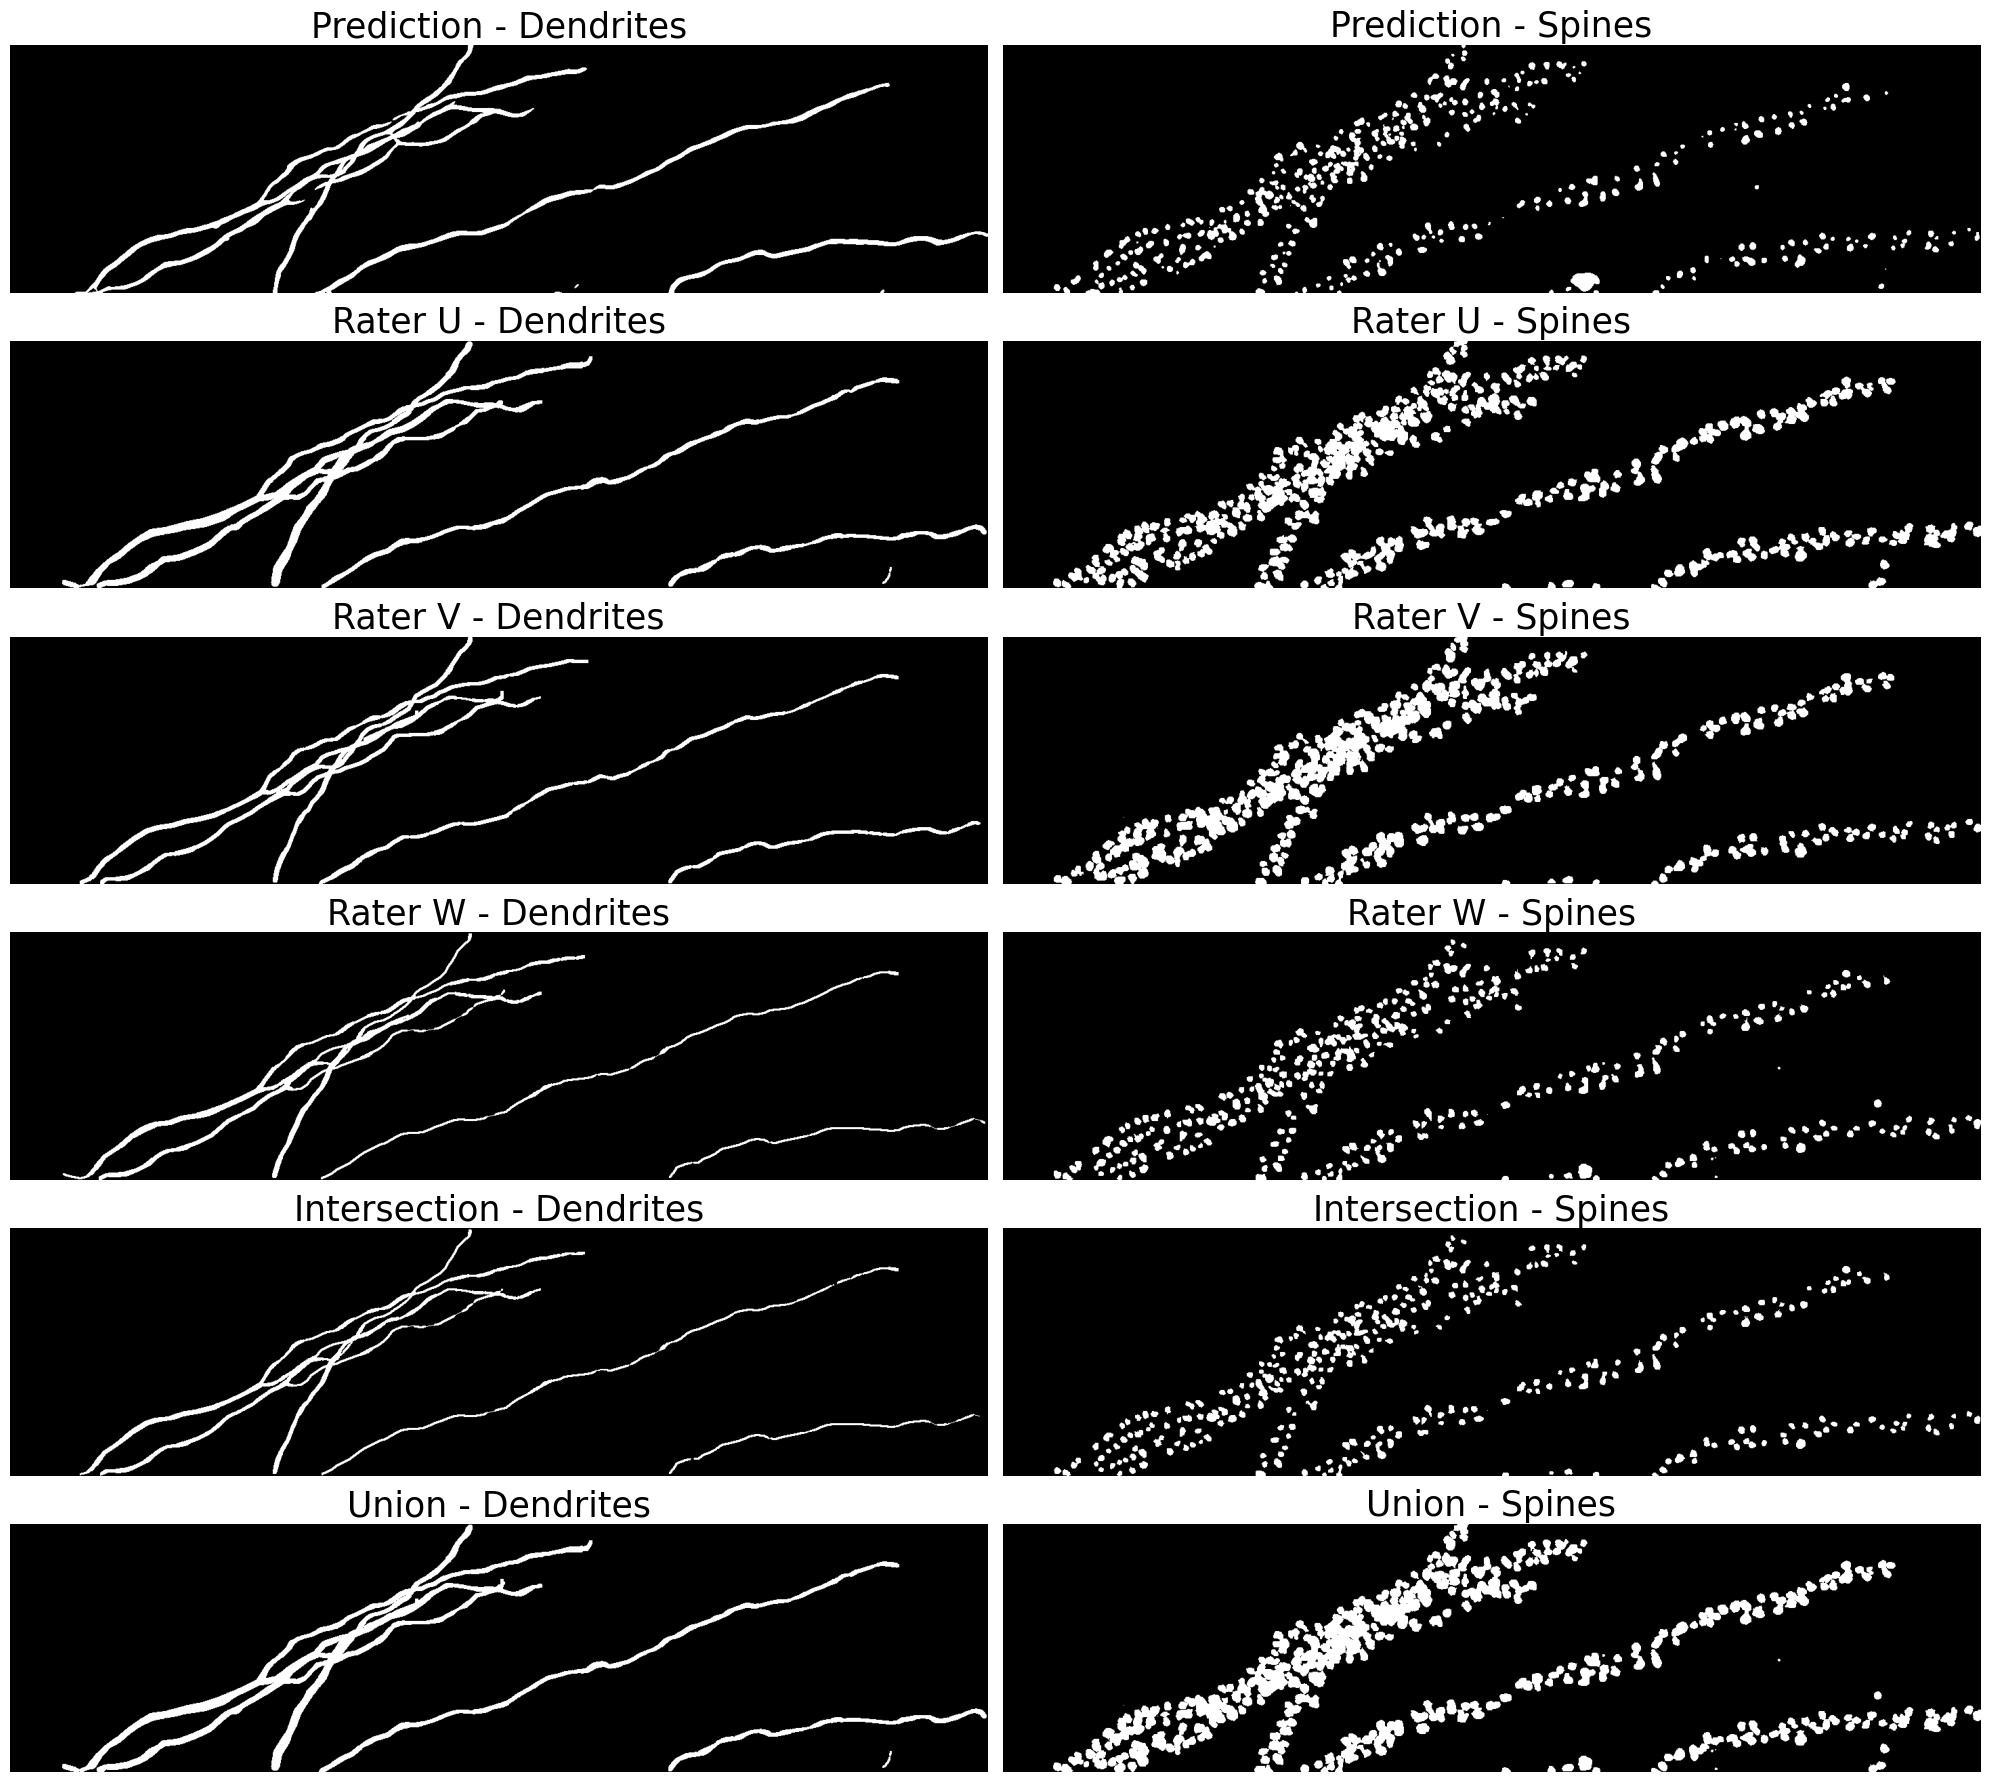
\includegraphics[width=0.95\textwidth]{figures/23_deepd3_qualitative.png}
\captionof{figure}{Qualitative comparison of \gls{DeepD3} predictions with individual rater annotations. Rows show the predicted masks, rater U, V, and W annotations, as well as intersection and union consensus masks. While dendrite predictions closely align across all references, spine annotations show notable differences in density and coverage. Scale: $0.94\,\mu\text{m}/\text{px}$}
\label{fig:deepd3_qualitative}
\end{center}

These results establish a strong empirical baseline for both dendrite and spine segmentation. In the following section, we evaluate the performance of \gls{SAM}-based approaches introduced in the Feature Work chapter.

\section{Segment Anything Model}
The \gls{SAM} model was evaluated on the benchmark dataset in both zero-shot and fine-tuned settings. Given its general-purpose design, \gls{SAM} was applied only to the task of \textit{dendrite segmentation}. For zero-shot inference, we used a grid-based prompting strategy, placing point prompts at regular intervals across the image plane. For fine-tuning, \gls{SAM} was tested using point prompts derived from \texttt{goodFeaturesToTrack} along the dendritic shaft, with overlapping patches extracted from the training volumes. All results presented in this section were obtained using the \texttt{\gls{ViT}-H} variant of \gls{SAM}.

A qualitative comparison of the raw benchmark stack, zero-shot predictions (grid size 16), and fine-tuned predictions is shown in \autoref{fig:sam_qualitative}. The zero-shot predictions exhibit sparse, patchy coverage and substantial noise. While some dendritic structures are partially identified, the segmentation lacks continuity and misses finer branches entirely. In contrast, the fine-tuned model produces denser masks with greater coverage of dendrite segments, though it still suffers from over-segmentation and grid-like artifacts related to patch-based inference.

\begin{center}
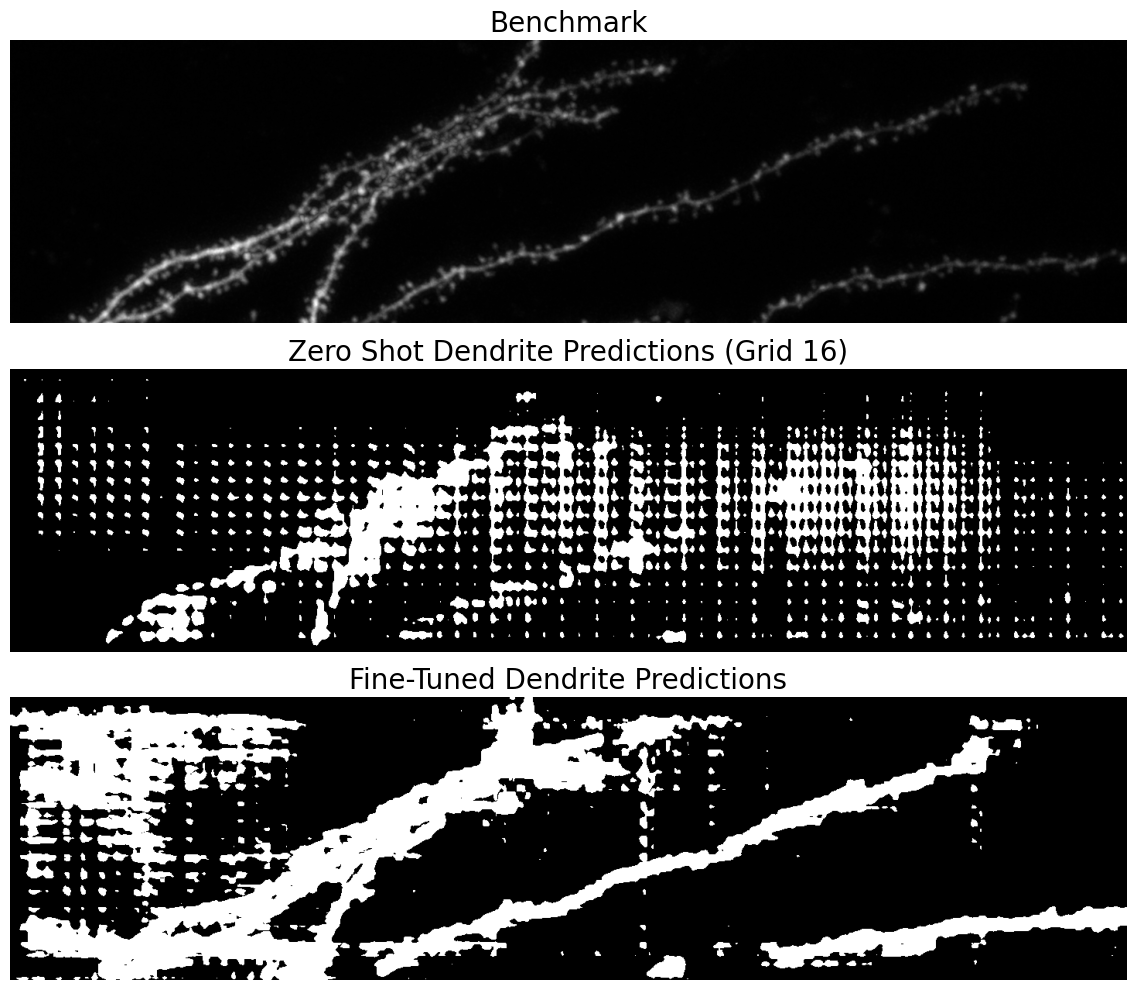
\includegraphics[width=0.8\textwidth]{figures/24_sam_qualitative.png}
\captionof{figure}{Qualitative comparison of \gls{SAM} predictions. Top: Raw benchmark image. Middle: Zero-shot prediction using grid size 16. Bottom: Prediction from fine-tuned \gls{SAM}. Zero-shot output is sparse and noisy, while fine-tuned results improve coverage but remain over-segmented. Scale: $0.94\,\mu\text{m}/\text{px}$}
\label{fig:sam_qualitative}
\end{center}

Quantitative results for the zero-shot \gls{SAM} setup are shown in \autoref{fig:sam_zeroshot_metrics}. Using grid-based point prompts, the best performance was observed at a grid size of 16, with a Dice score of 0.248 and an \gls{IoU} of 0.141 against rater U. At coarser grid sizes (32 and above), the model failed to produce any coherent segmentation, yielding near-zero scores. This poor performance can be attributed to the fact that grid prompts are spatially uniform and semantically uninformed. Since \gls{SAM} relies heavily on prompt relevance to generate accurate masks, indiscriminate prompting across the image leads to fragmented and noisy outputs, especially in dense and ambiguous biomedical scenes like dendrites.

\begin{center}
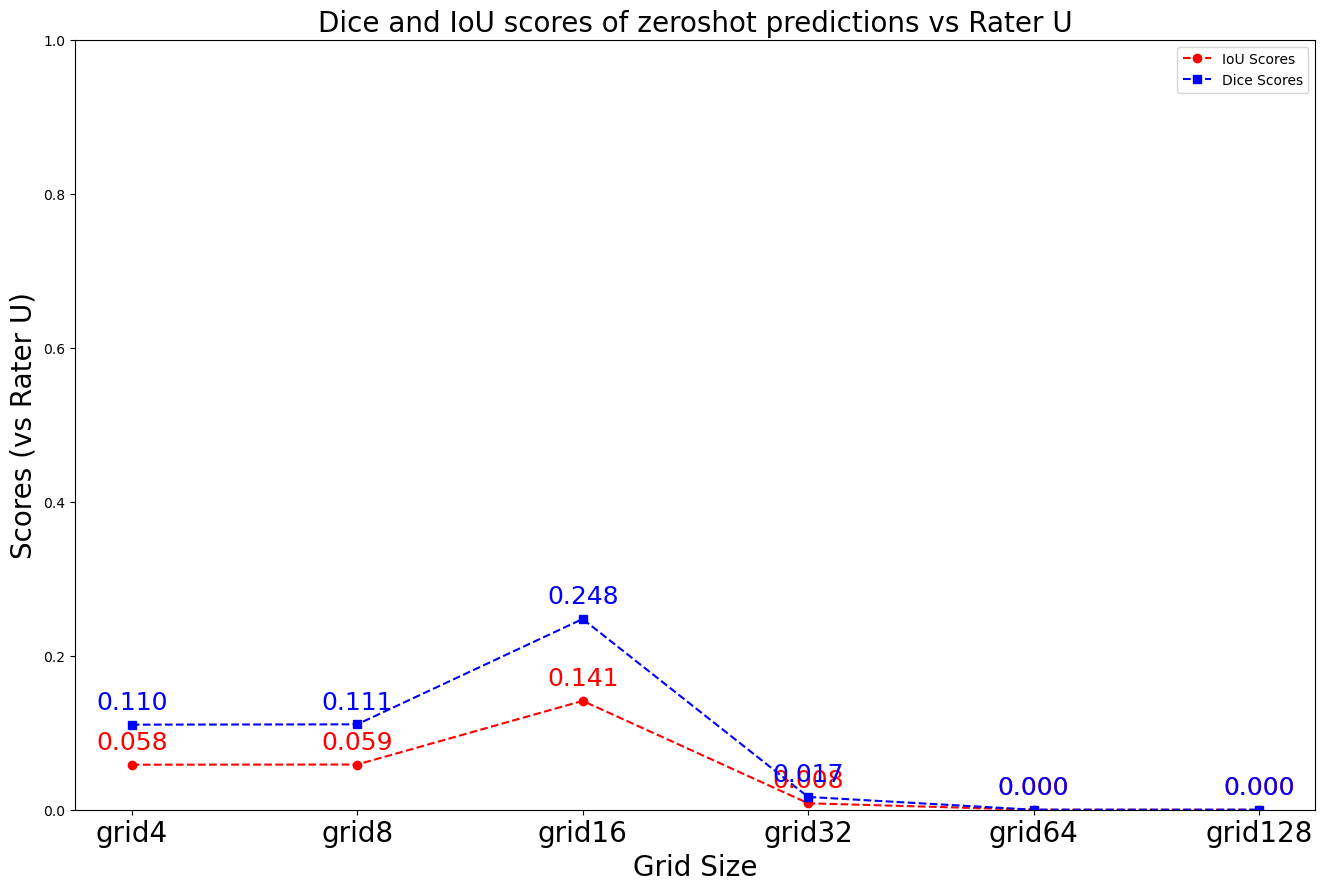
\includegraphics[width=0.8\textwidth]{figures/25_sam_zeroshot_metrics.png}
\captionof{figure}{Zero-shot \gls{SAM} dendrite segmentation performance. Dice and \gls{IoU} scores across different grid sizes using grid-based point prompts, evaluated against rater U. Performance peaks at grid size 16, but remains very bad overall, highlighting the ineffectiveness of prompt-agnostic zero-shot inference for this task.}
\label{fig:sam_zeroshot_metrics}
\end{center}

To address these limitations, the model was fine-tuned on task-specific dendritic data using tracked feature points as prompts. As shown in \autoref{fig:sam_finetuned_metrics}, fine-tuning substantially improved segmentation quality. The highest Dice and \gls{IoU} scores were observed against the union mask, reaching 0.341 and 0.205, respectively. Performance dropped when compared with intersection mask, where Dice and \gls{IoU} fell to 0.203 and 0.113. This spread reflects the continued sensiti\gls{ViT}y of the model to prompt quality and ground truth ambiguity. While fine-tuning helped the model learn contextual cues and reduced noise, the predictions still exhibited grid artifacts and lacked precision around dendritic boundaries. Nevertheless, the improvement over the zero-shot variant establishes the importance of task-specific adaptation even for powerful foundation models like \gls{SAM}.

\begin{center}
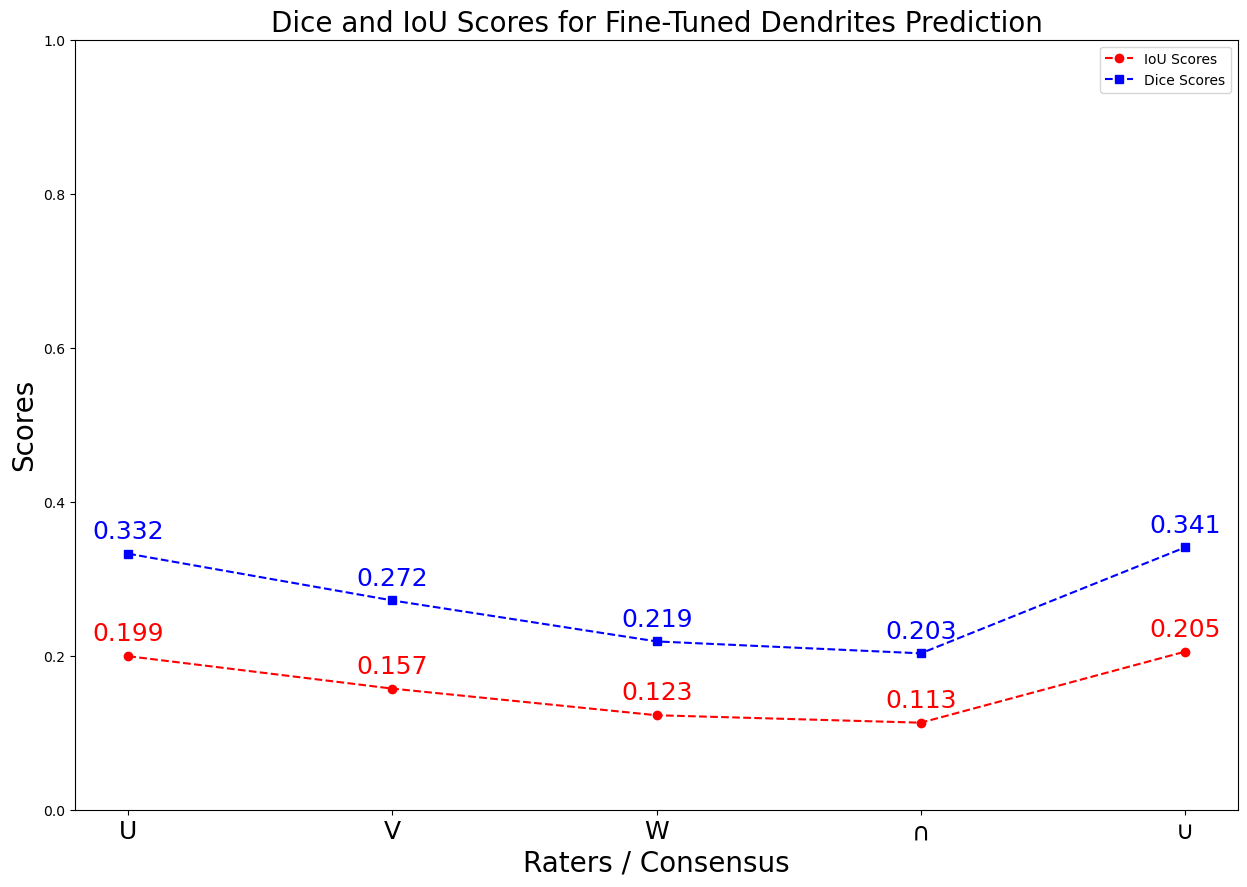
\includegraphics[width=0.8\textwidth]{figures/26_sam_finetuned_metrics.png}
\captionof{figure}{Fine-tuned \gls{SAM} dendrite segmentation performance. Dice and \gls{IoU} scores evaluated against three individual raters and consensus masks. Fine-tuning improves performance substantially over zero-shot \gls{SAM}, though results still vary depending on the reference mask.}
\label{fig:sam_finetuned_metrics}
\end{center}

These results demonstrate that while \gls{SAM} possesses general segmentation capabilities, it fails to perform reliably on dendritic structures without task-specific adaptation. Fine-tuning improves segmentation quality but remains insufficient for precise and consistent dendrite segmentation. This motivated the exploration of parameter-efficient fine-tuning strategies such as Low Rank Adaptation.

\section{SAM with Low-Rank Adaptation}
While the fine-tuned \gls{SAM} model showed moderate improvements over zero-shot performance, its outputs remained noisy and prone to over-segmentation. To improve generalization while maintaining training efficiency, we leveraged \gls{LoRA} to fine-tune \gls{SAM} on the dendrite segmentation task. \gls{LoRA} introduces task-specific trainable matrices into frozen transformer weights, significantly reducing the number of learnable parameters while preserving model capacity. Based on the failure of prompt-agnostic zero-shot \gls{SAM}, we directly adopted a fine-tuned \gls{LoRA} setup, avoiding zero-shot evaluation entirely.

A qualitative example comparing the benchmark image and \gls{SAM} + \gls{LoRA} predictions is shown in \autoref{fig:lora_qualitative}. Compared to both zero-shot and fully fine-tuned \gls{SAM}, \gls{LoRA} predictions demonstrate stronger continuity along dendritic shafts, reduced noise, and better adherence to structural boundaries. Visual artifacts observed in earlier variants, such as over-segmentation and patch-induced grid effects, are substantially minimized.

\begin{center}
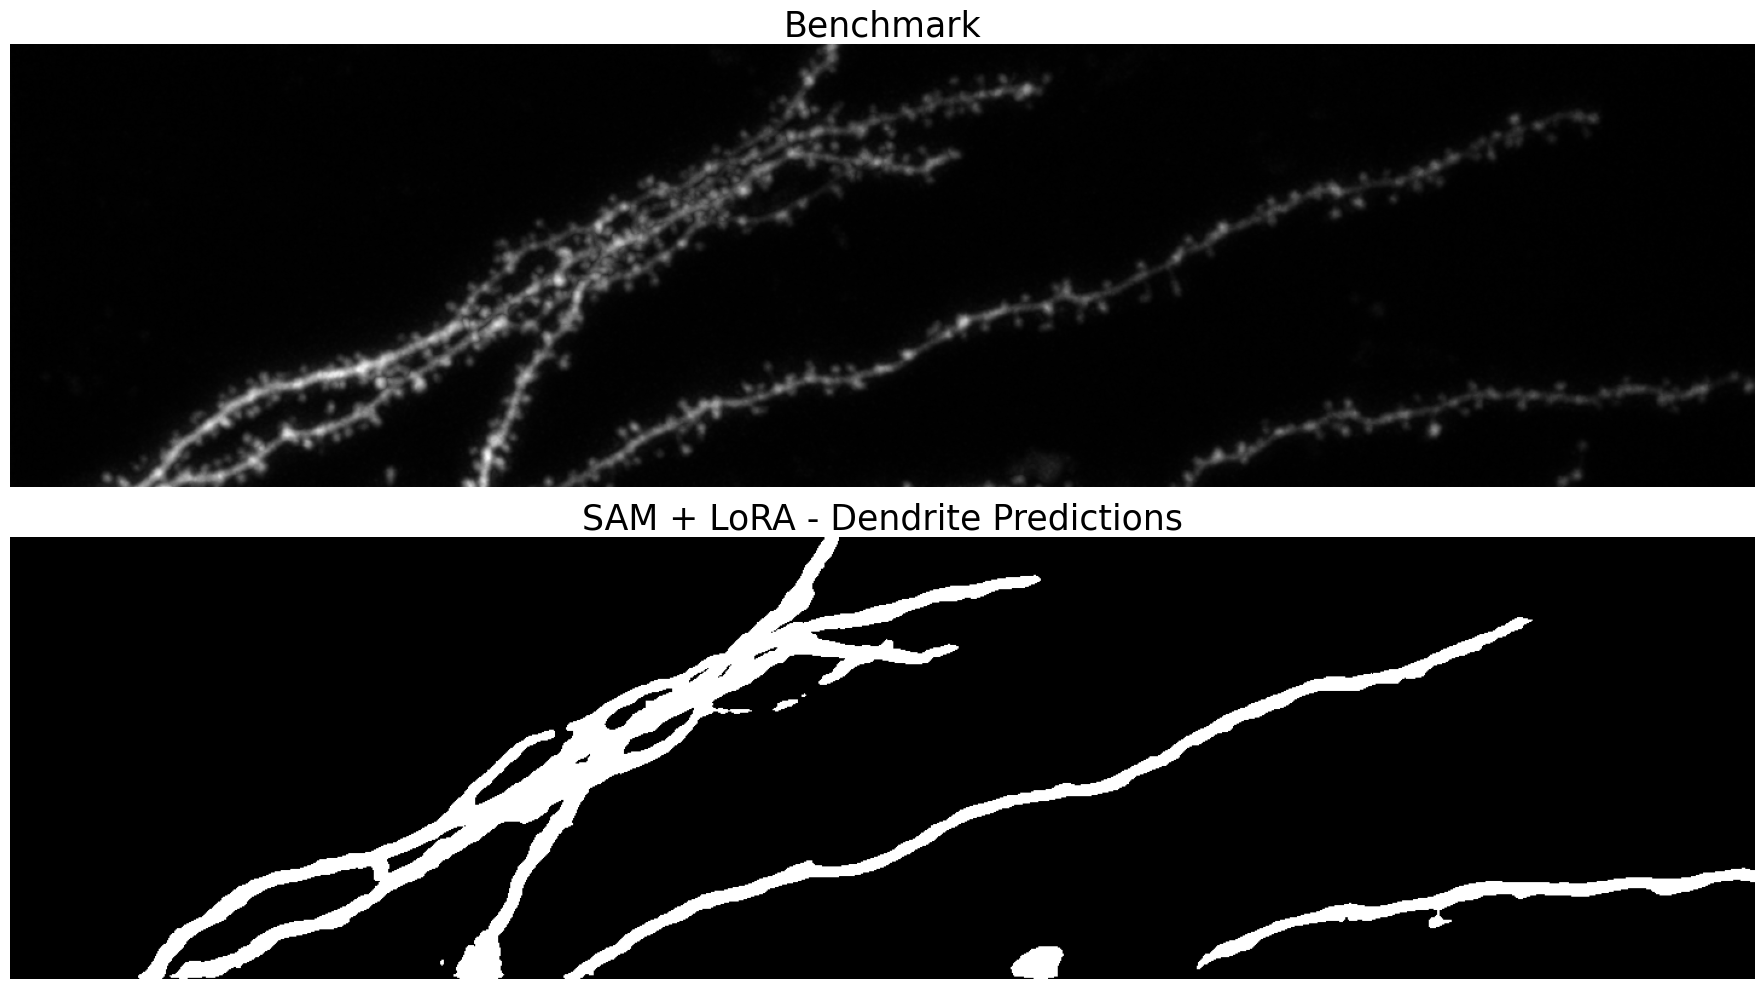
\includegraphics[width=0.9\textwidth]{figures/27_lora_qualitative.png}
\captionof{figure}{Qualitative dendrite segmentation using \gls{SAM} + \gls{LoRA}. Top: Raw benchmark image. Bottom: Prediction using \gls{SAM} + \gls{LoRA}. The model produces clean, continuous segmentation masks with reduced background noise and improved shaft delineation. Scale: $0.94\,\mu\text{m}/\text{px}$}
\label{fig:lora_qualitative}
\end{center}

\begin{center}
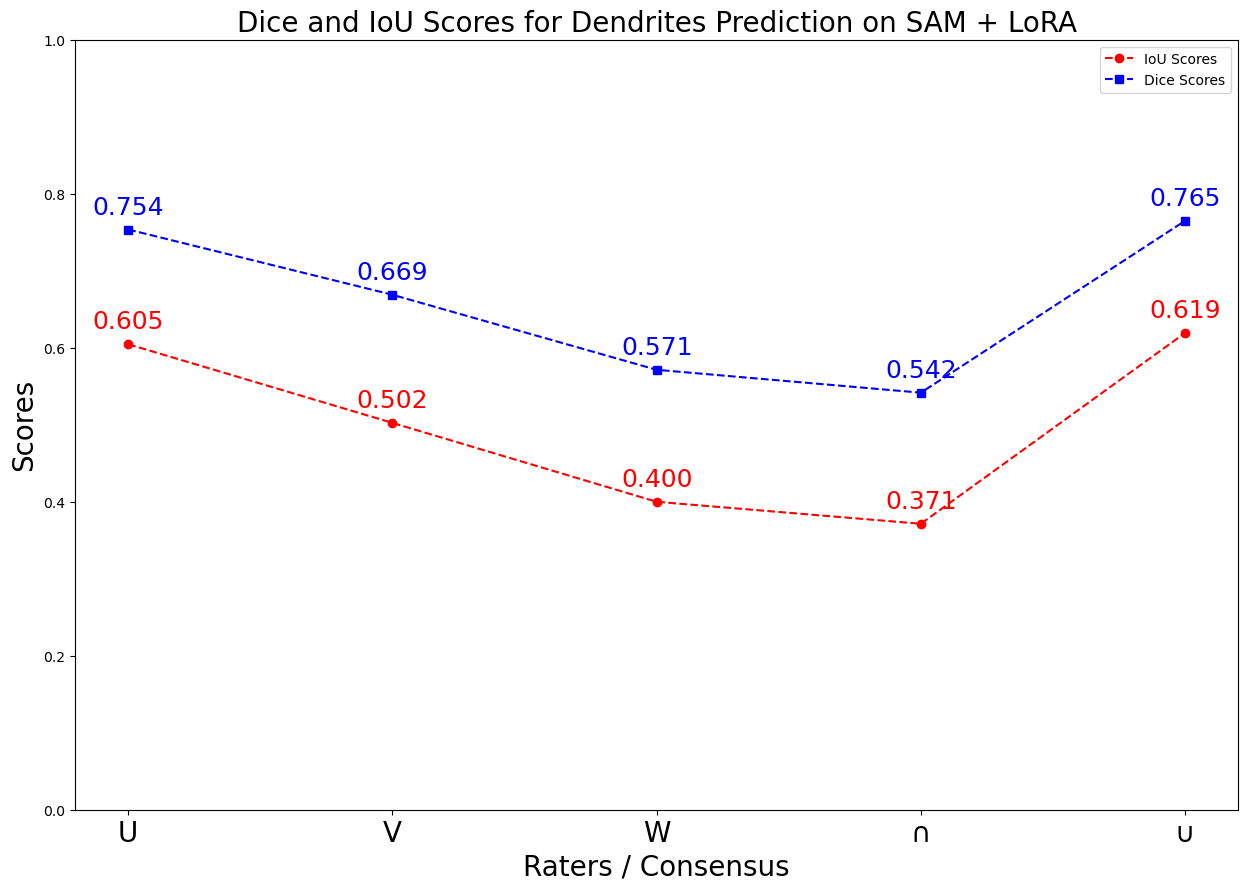
\includegraphics[width=0.8\textwidth]{figures/28_lora_metrics.png}
\captionof{figure}{Dice and \gls{IoU} scores for \gls{SAM} + \gls{LoRA} dendrite segmentation. Evaluation against individual raters and consensus masks. \gls{LoRA} shows consistent improvements over both zero-shot and fully fine-tuned \gls{SAM}. Scale: $0.94\,\mu\text{m}/\text{px}$}
\label{fig:lora_metrics}
\end{center}


Quantitatively, \gls{SAM} + \gls{LoRA} outperforms both the zero-shot and fully fine-tuned \gls{SAM} variants across all raters and consensus masks, as shown in \autoref{fig:lora_metrics}. The model achieves a maximum Dice score of 0.765 and \gls{IoU} of 0.619 when evaluated against the union mask. Even against stricter references such as the intersection mask, performance remains high, with Dice and \gls{IoU} scores of 0.542 and 0.371, respectively. These consistent improvements confirm that \gls{LoRA}-based fine-tuning enhances both mask quality and generalization without incurring the instability of full model training.

To further assess qualitative differences, we compared frame-level predictions across methods. \autoref{fig:lora_framewise_comparison} shows predictions for two representative slices (Frame 23 and 36). \gls{SAM} + \gls{LoRA} more accurately captures dendritic continuity and fine detail compared to \gls{DeepD3}, while also avoiding the patch-based artifacts that degraded \gls{SAM}’s outputs. These results reinforce \gls{LoRA}’s effectiveness in enabling stable, parameter-efficient fine-tuning tailored to the structural characteristics of dendrites.

\begin{center}
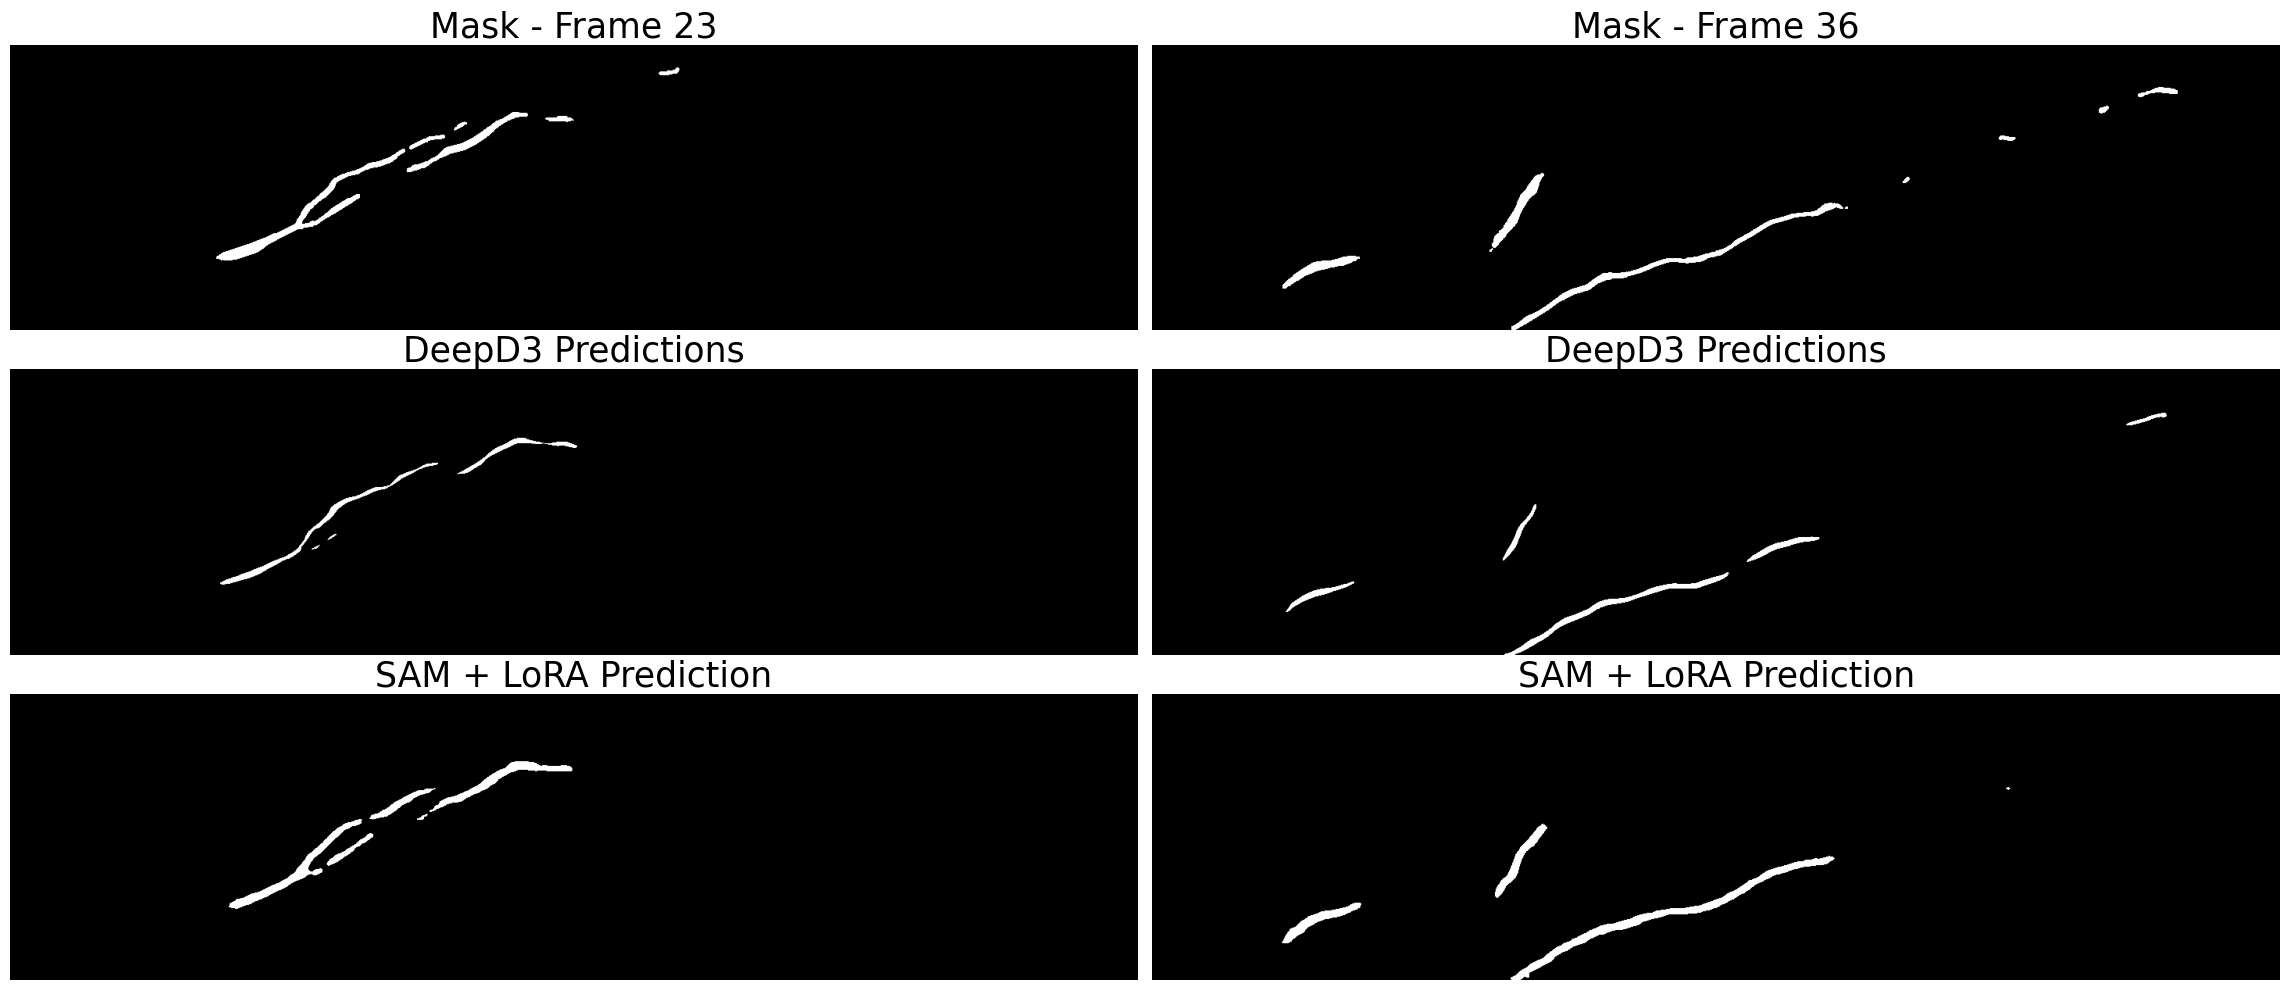
\includegraphics[width=0.95\textwidth]{figures/29_lora_framewise_comparison.png}
\captionof{figure}{Frame-wise comparison across models. Top: Ground truth masks for Frames 23 and 36. Middle: \gls{DeepD3} predictions. Bottom: \gls{SAM} + \gls{LoRA} predictions. \gls{LoRA} outputs display better structural continuity and less fragmentation than \gls{DeepD3}, and fewer artifacts than standard \gls{SAM}. Scale: $0.94\,\mu\text{m}/\text{px}$}
\label{fig:lora_framewise_comparison}
\end{center}

Overall, \gls{SAM}+\gls{LoRA} serves as a strong middle ground between zero-shot generalization and full-model fine-tuning, offering improved performance with fewer learnable parameters. These findings build a strong case for its use in domain-adapted segmentation pipelines, especially when working with limited annotations. Its balance of efficiency and accuracy makes \gls{SAM}+\gls{LoRA} particularly well-suited for neuroimaging tasks where dense annotations are costly. These advantages set the stage for our final and most comprehensive system: Neuro-\gls{SAM}.

\section{Neuro-SAM}
Neuro-\gls{SAM} is the final modular framework proposed in this thesis, designed to overcome the limitations observed in earlier \gls{SAM}-based approaches. Instead of building directly on previous variants like \gls{SAM} or \gls{SAM}+\gls{LoRA}, Neuro-\gls{SAM} leverages insights gained from those experiments to construct a more robust and task-specific pipeline powered by \gls{SAMv2}. The complete system consists of four interlinked modules: a waypoint-aware path tracing module, a \gls{SAMv2}-based dendrite segmentation module, a dual-view spine detection module, and a localized spine segmentation module. In this section, we evaluate the performance of each module independently, demonstrating the improvements achieved across dendrite and dendritic spine segmentation tasks.

\subsection{Path Tracing Module}
Accurate dendrite path tracing is a foundational step in Neuro-\gls{SAM}, enabling precise downstream segmentation and analysis. Manual tracing is both time-consuming and prone to subjective bias, particularly in dense or noisy regions. To address this, we developed a waypoint-aware path tracing module built upon a customized version of brightest-path-lib \cite{Jha_2023}. By allowing users to define start, end, and optional waypoint points, the module can robustly trace complex dendrite geometries with minimal input. This interactive tracing approach offers both control and automation, making it highly effective across a range of morphologies and image conditions.

\begin{center}
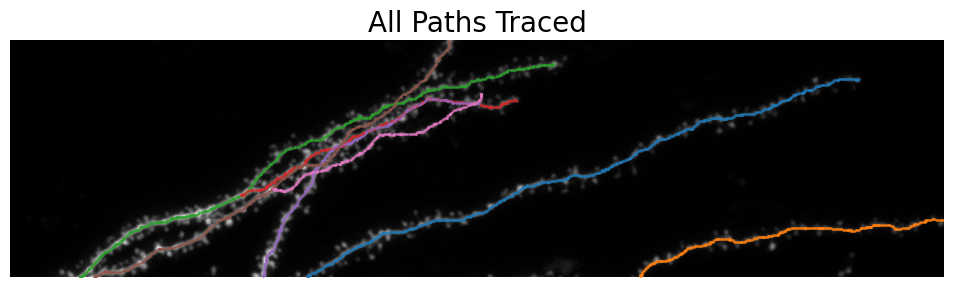
\includegraphics[width=1.0\textwidth]{figures/30_path_overview.png}
\captionof{figure}{Overview of traced dendritic paths. Multiple dendrites traced using the path tracing module of Neuro-\gls{SAM}. Each color represents an independently traced dendrite, demonstrating the module's robustness across diverse geometries and imaging conditions. Scale: $0.94\,\mu\text{m}/\text{px}$}
\label{fig:path_overview}
\end{center}

The path tracing module in Neuro-\gls{SAM} enables users to effortlessly trace complex dendritic structures by specifying just a start point, an end point, and optionally, a sparse set of waypoints. \autoref{fig:path_overview} illustrates a collection of traced dendritic paths over the benchmark stack, demonstrating the system's ability to handle diverse curvatures, crossings, and branch orientations. As shown in \autoref{fig:path_waypoints}, even challenging trajectories can be recovered with high spatial precision using minimal supervision. The waypoint-guided formulation allows flexible course correction in ambiguous regions, ensuring accurate adherence to the dendrite centerline without manual pixel-level editing. This capability not only streamlines user interaction but also produces reliable paths for downstream segmentation tasks.

\begin{center}
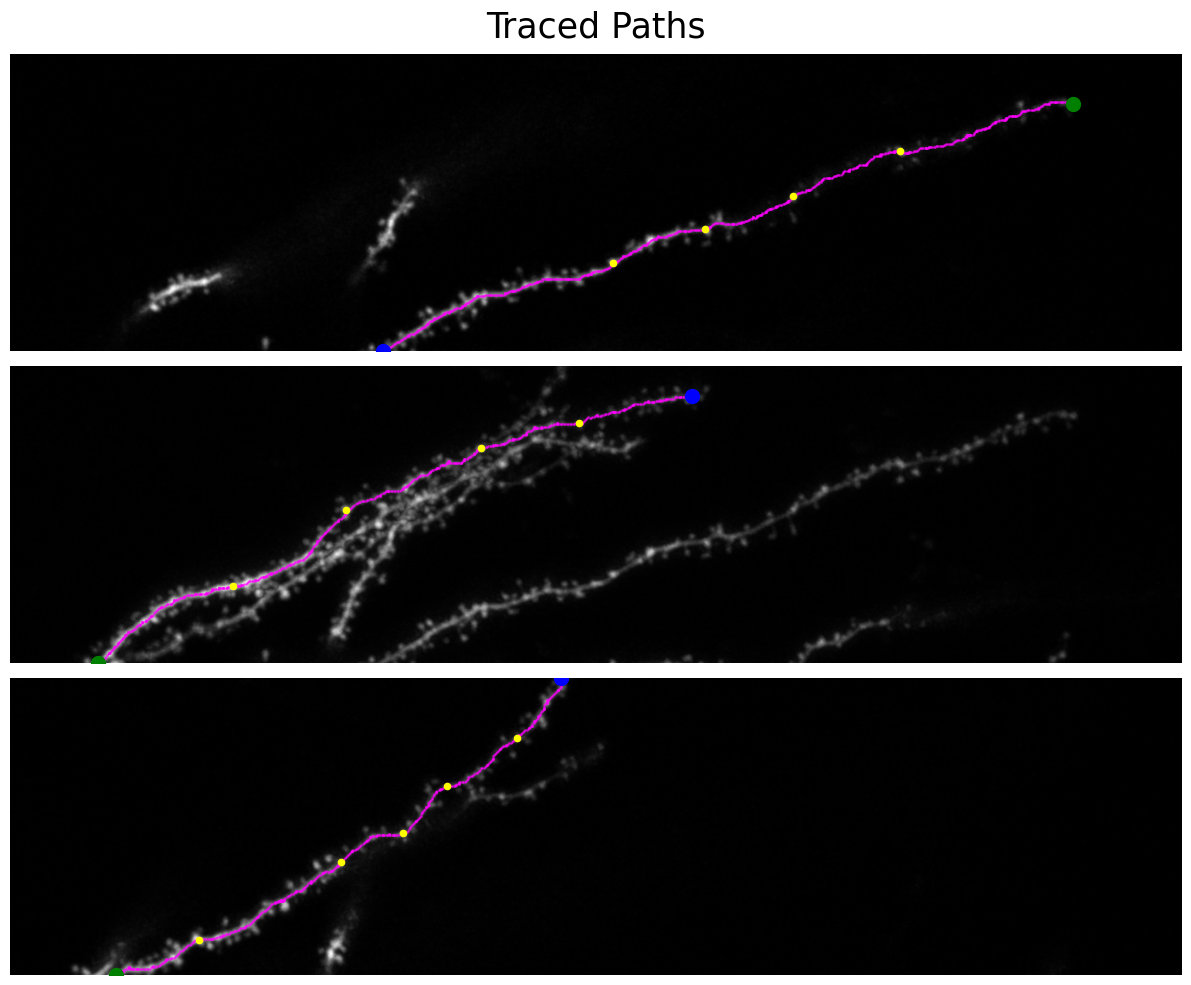
\includegraphics[width=0.8\textwidth]{figures/31_path_waypoints.png}
\captionof{figure}{Waypoint-guided path tracing. Example traces generated using the Neuro-\gls{SAM}'s path tracing module. Blue, green, and yellow dots represent start points, end points, and user-defined waypoints, respectively. Scale: $0.94\,\mu\text{m}/\text{px}$}
\label{fig:path_waypoints}
\end{center}

\subsubsection{\textbf{Comparison with brightest-path-lib}}
To evaluate the improvements introduced by our modified path tracing module, we compared its output to the original brightest-path-lib \cite{Jha_2023}, which computes optimal paths solely between two endpoints using voxel intensities. While the original method often produces valid traces in simple regions, it struggles in densely packed or twisted dendritic structures, frequently deviating from the true centerline or jumping across nearby branches. In contrast, Neuro-\gls{SAM}'s path tracing module provides local guidance at critical turning points, effectively constraining the search space and enabling more biologically plausible trajectories. Qualitatively, our module produces smoother, anatomically consistent paths with significantly fewer deviations or misroutes.

\begin{center}
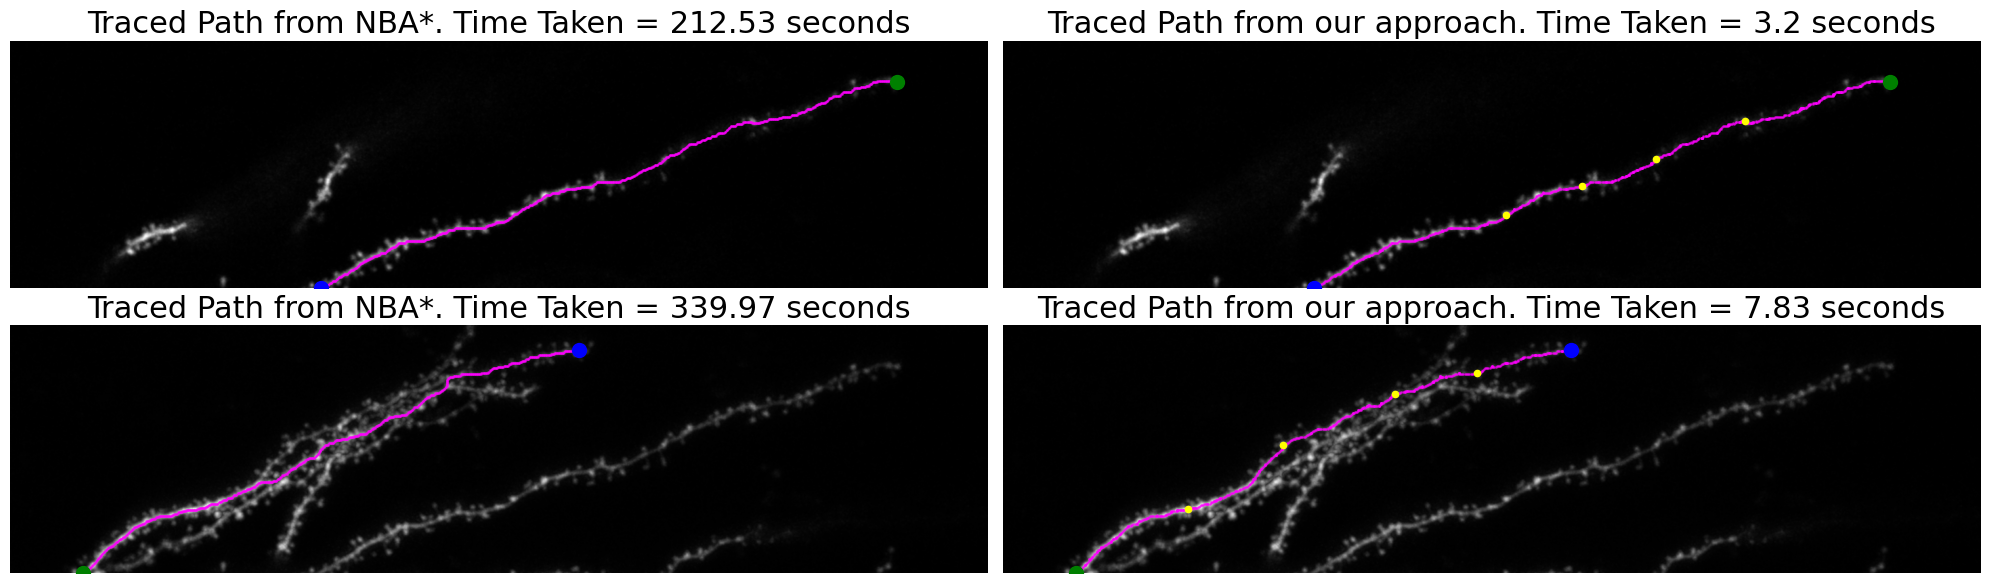
\includegraphics[width=0.95\textwidth]{figures/32_path_comparison.png}
\captionof{figure}{Comparison of dendrite path tracing: NBA* vs Neuro-\gls{SAM}. Traces generated using the original brightest-path-lib (left) and our modified waypoint-aware module (right). Scale: $0.94\,\mu\text{m}/\text{px}$}
\label{fig:path_comparison}
\end{center}

\subsection{Segmentation Module}

Following path tracing, the segmentation module in Neuro-\gls{SAM} performs segmentation of dendrite shafts using a refined adaptation of \gls{SAMv2}. Unlike earlier models that relied on generic grid prompts or local feature points, our pipeline leverages the traced dendrite path to sample overlapping patches and extract precise, geometry-aware prompts. This path-conditioned prompting strategy allows Neuro-\gls{SAM} to generate spatially coherent segmentations even in regions with low contrast, occlusions, or complex curvature. The segmentation model was trained on high-resolution volumes with custom prompt tuning and inference postprocessing, ensuring robustness across multiple datasets.

\begin{center}
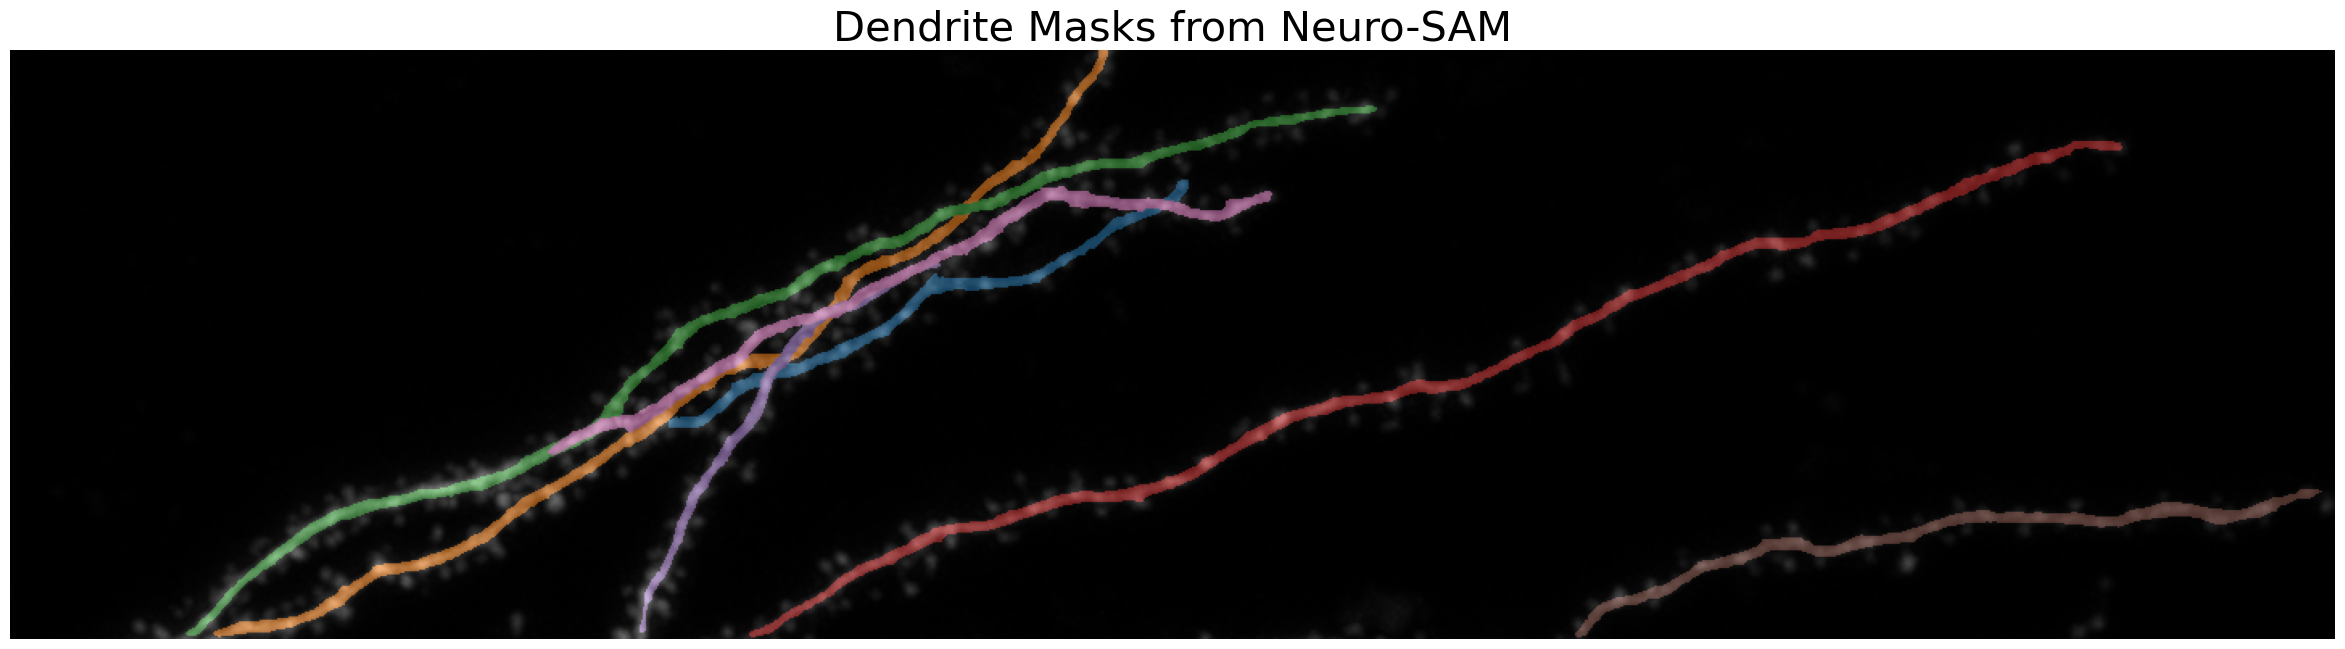
\includegraphics[width=0.95\textwidth]{figures/33_dendrite_seg_all.png}
\captionof{figure}{Predicted dendrite masks from Neuro-\gls{SAM} overlaid on the benchmark stack. Each dendritic shaft is segmented individually and visualized in different colours. Scale: $0.94\,\mu\text{m}/\text{px}$}
\label{fig:dendrite_seg_all}
\end{center}

The segmentation results from Neuro-\gls{SAM} exhibit highly accurate dendritic masks, closely following the underlying morphology traced in the benchmark image stack. As shown in \autoref{fig:dendrite_seg_all}, each dendrite is individually segmented and rendered with clear boundaries, even in curved regions and near other dendrites. The ability to isolate individual shafts across the 3D stack ( \autoref{fig:separate_masks}) further confirms the spatial coherence and continuity achieved by our path-conditioned prompting strategy.

\begin{center}
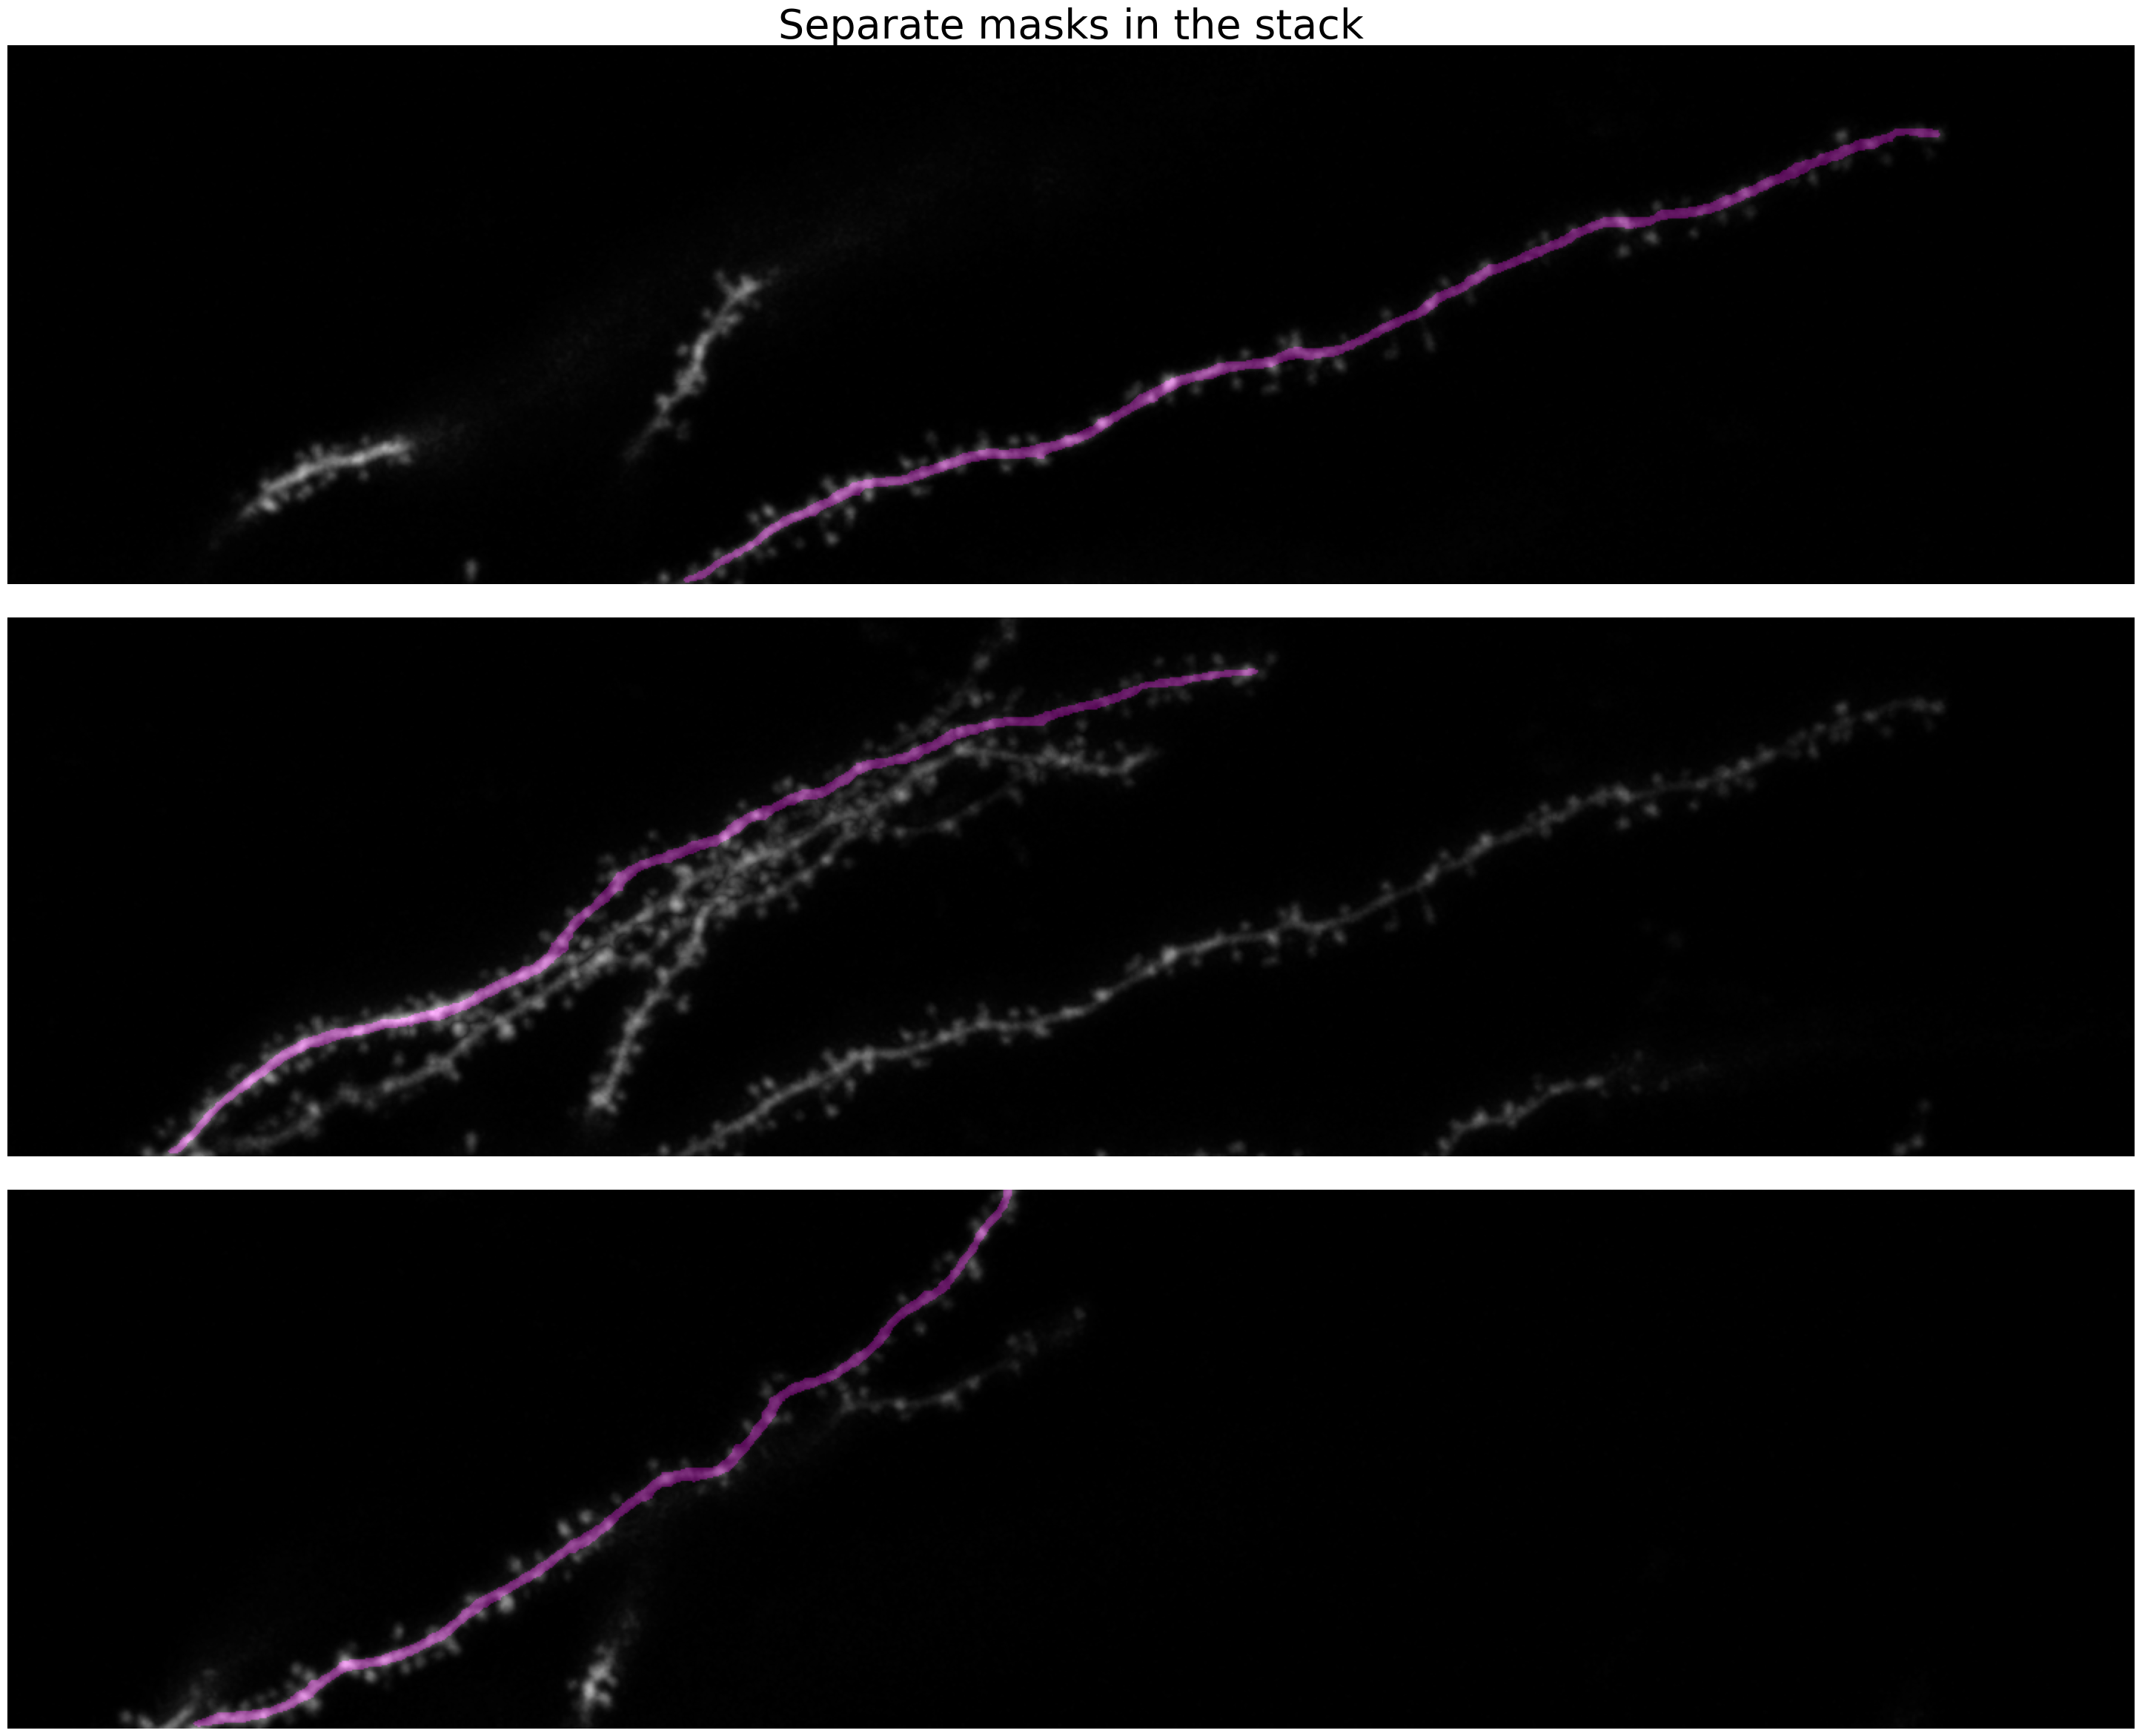
\includegraphics[width=0.9\textwidth]{figures/34_separate_masks.png}
\captionof{figure}{Individual dendrite segmentations from Neuro-\gls{SAM} shown across different regions of the stack. Scale: $0.94\,\mu\text{m}/\text{px}$}
\label{fig:separate_masks}
\end{center}

\begin{center}
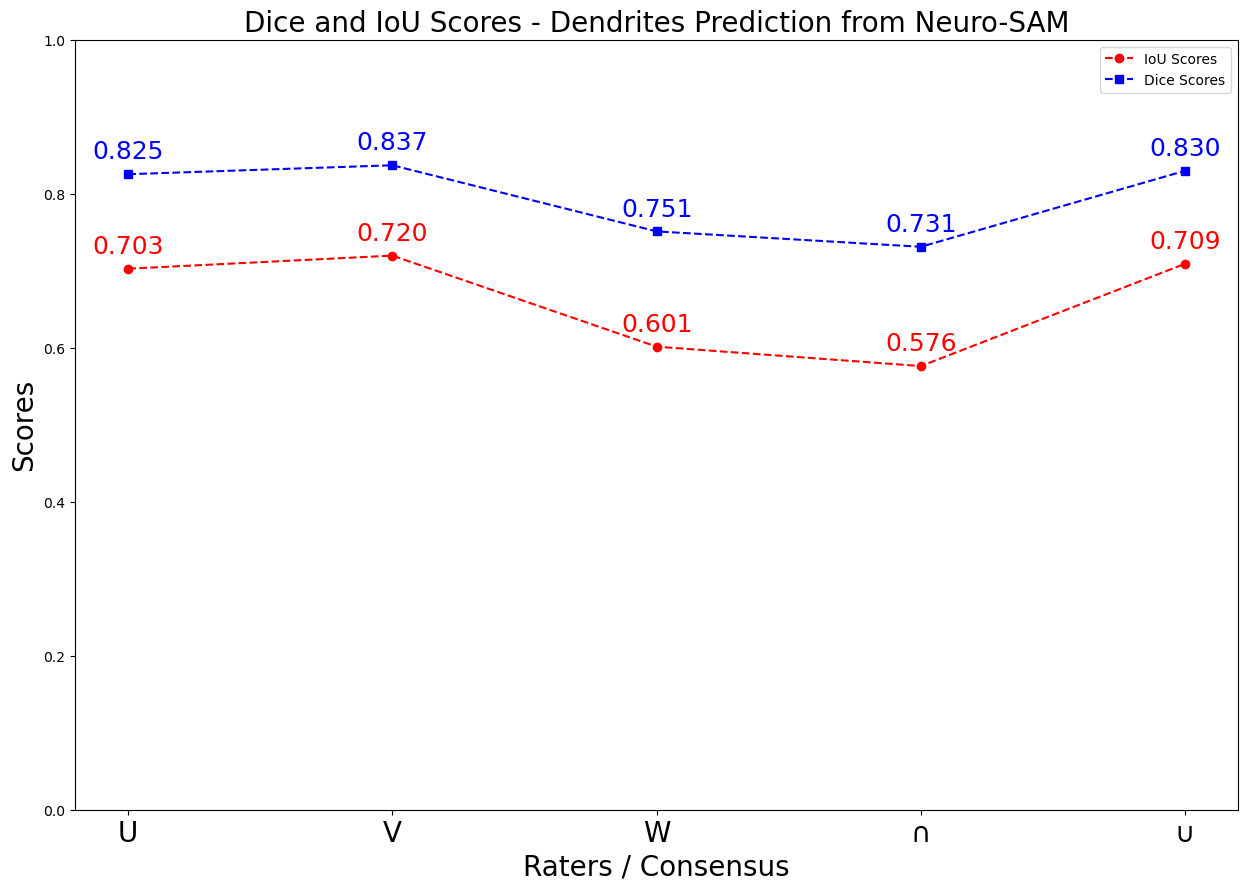
\includegraphics[width=0.7\textwidth]{figures/35_dendrite_metric_neurosam.png}
\captionof{figure}{Dice and \gls{IoU} scores for dendrite predictions from Neuro-\gls{SAM} across different raters and consensus masks.}
\label{fig:dendrite_metric_neurosam}
\end{center}

As visualized in \autoref{fig:dendrite_metric_neurosam}, Neuro-\gls{SAM} achieves consistently high Dice and \gls{IoU} scores across all raters and consensus annotations, with Dice values reaching up to 0.837 and \gls{IoU} up to 0.720. These numbers significantly outperform prior variants, including base \gls{SAM}, \gls{SAM}+\gls{LoRA} and \gls{DeepD3}, demonstrating the effectiveness of our prompt tuning and training strategy. The low variance across raters also indicates stable generalization across inter-rater variability and imaging conditions.



\begin{center}
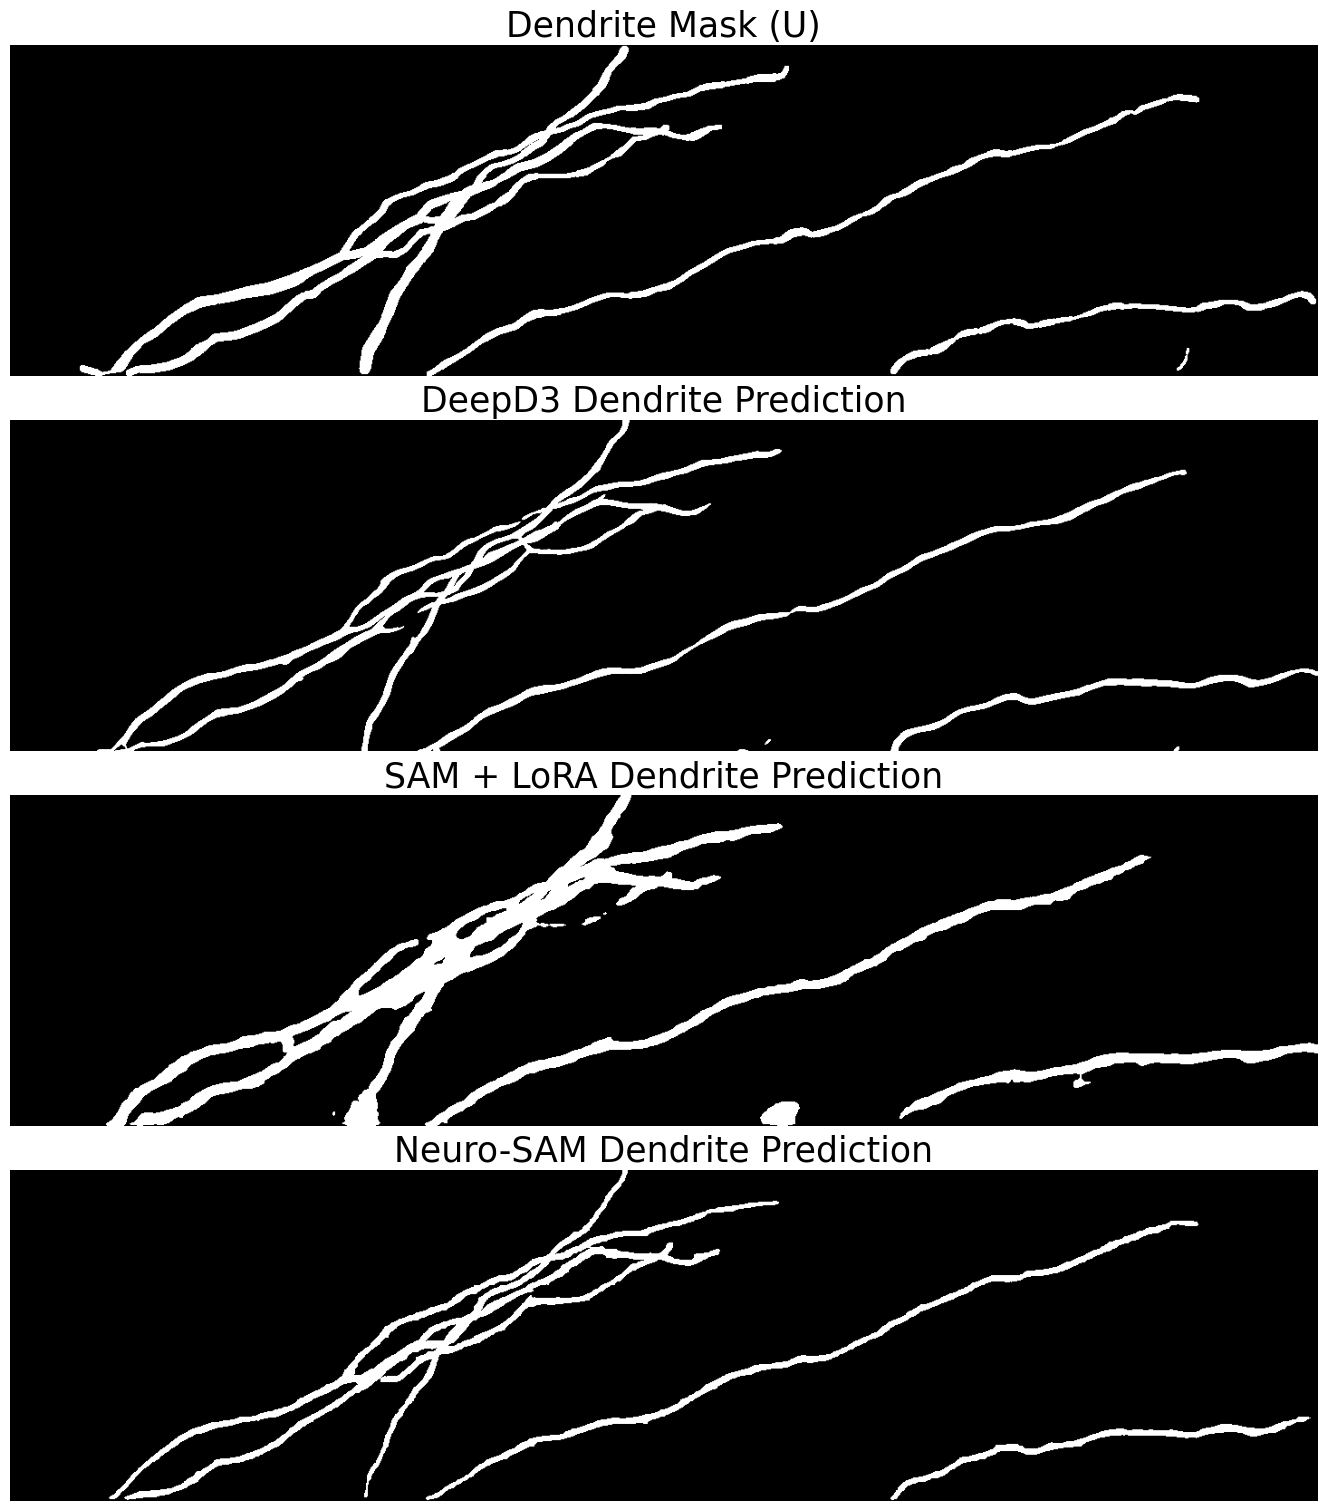
\includegraphics[width=0.65\textwidth]{figures/36_dendrite_compare_mask.png}
\captionof{figure}{Qualitative comparison of dendrite predictions from \gls{DeepD3}, \gls{SAM}+\gls{LoRA}, and Neuro-\gls{SAM} against the rater U mask. Neuro-\gls{SAM} demonstrates improved completeness and accuracy of segmentation, particularly in overlapping dendrites. Scale: $0.94\,\mu\text{m}/\text{px}$}
\label{fig:dendrite_compare_mask}
\end{center}

The comparative plot in \autoref{fig:dendrite_compare_mask} highlights the improvement of Neuro-\gls{SAM} over \gls{DeepD3} and \gls{SAM}+\gls{LoRA}. While \gls{DeepD3} captures overall structure, it often exhibits disconnected segments and under-segmentation in thinner regions. \gls{SAM}+\gls{LoRA}, though denser, tends to over-segment and merge adjacent shafts. In contrast, Neuro-\gls{SAM} provides precise, well-delimited masks that remain faithful to the ground truth. This is further reinforced in per-frame comparisons (\autoref{fig:compare_frame_masks}), where Neuro-\gls{SAM} reliably segments long dendritic stretches with better spatial continuity and fewer artifacts. It not only segments the dendrites better but with the help of Path Tracing algorithm, it even traces the dendrite regions that are often lacking in the masks but visible to the human eye. 

\begin{center}
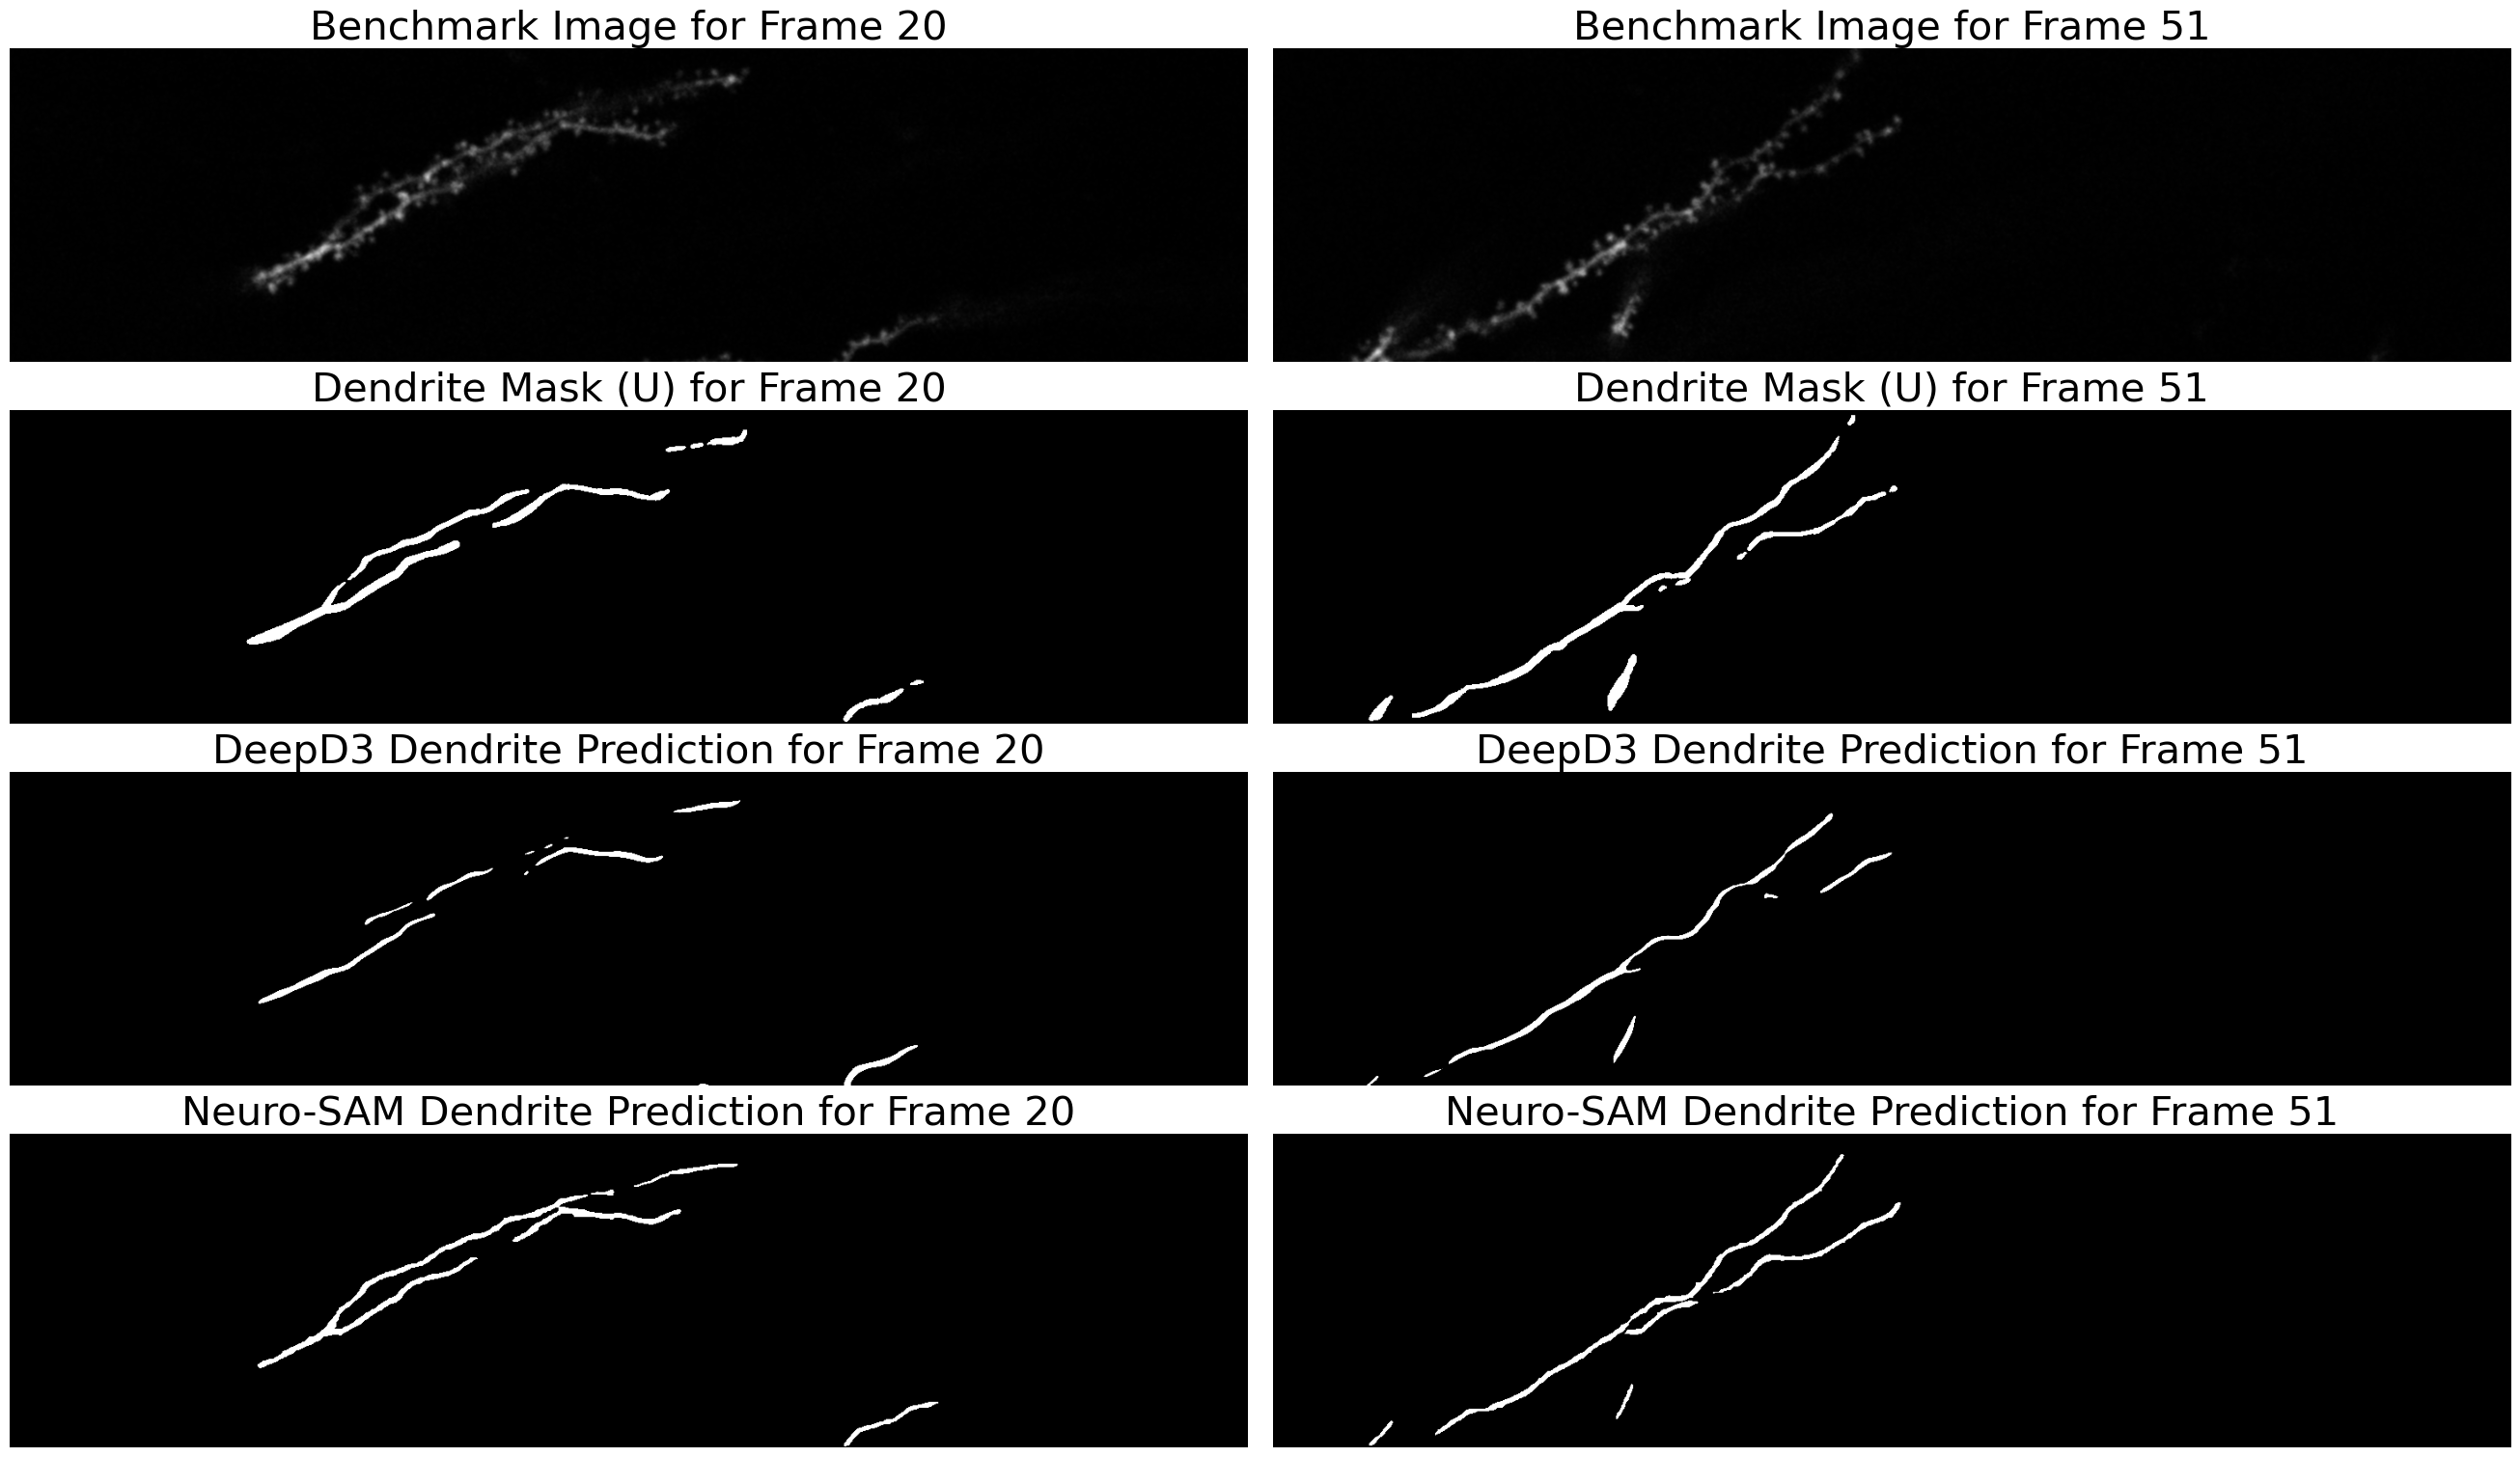
\includegraphics[width=0.95\textwidth]{figures/37_compare_frame_masks.png}
\captionof{figure}{Frame-wise comparison of dendrite predictions on benchmark images at timepoints 20 and 51. Neuro-\gls{SAM} consistently provides more complete and precise segmentations compared to \gls{DeepD3}, with better adherence to ground truth masks. Scale: $0.94\,\mu\text{m}/\text{px}$}
\label{fig:compare_frame_masks}
\end{center}

To contextualize performance, we compared Neuro-\gls{SAM} against \gls{DeepD3} across all raters and consensus masks. As shown in \autoref{fig:dendrite_metrics_comparison}, Neuro-\gls{SAM} consistently achieves slightly higher Dice and \gls{IoU} scores across all evaluations. These gains can be attributed to its geometry-aware prompting and tight integration with the traced path, which enhances mask continuity and alignment with dendritic morphology. In contrast, \gls{DeepD3} exhibits good performance but shows occasional fragmentation or missed segments, particularly in low-contrast or overlapping regions.

\begin{center}
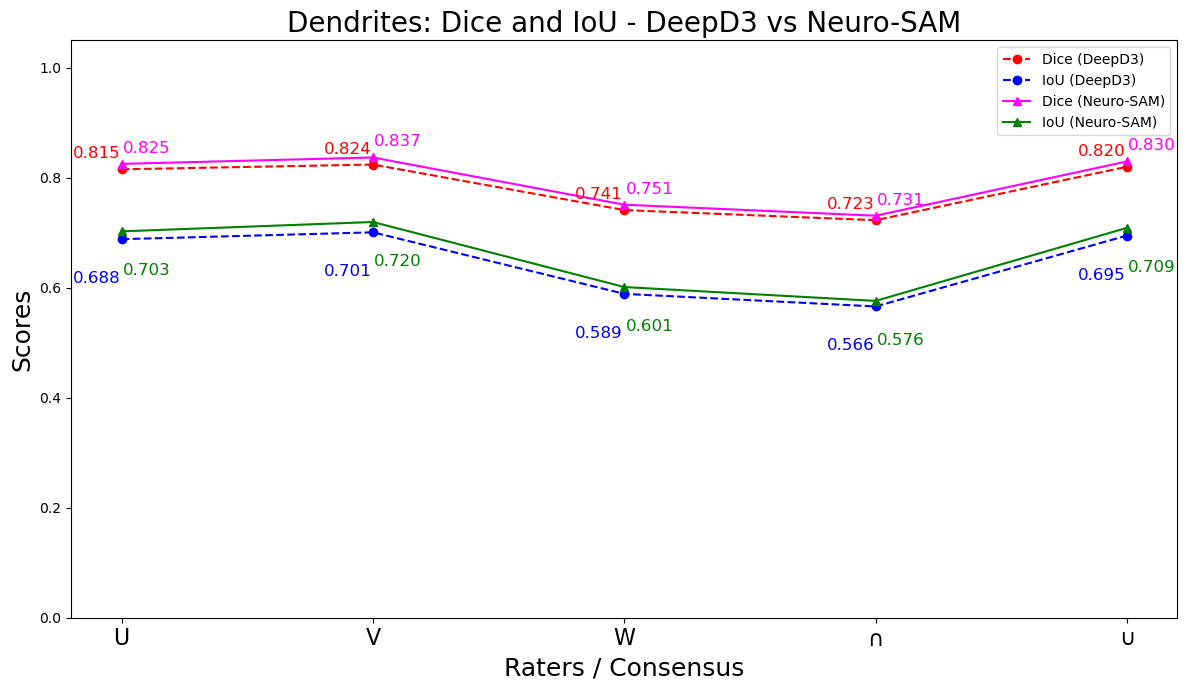
\includegraphics[width=0.9\textwidth]{figures/45_dendrite_metrics_comparison.png}
\captionof{figure}{Quantitative comparison of dendrite segmentation performance between \gls{DeepD3} and Neuro-\gls{SAM}. Neuro-\gls{SAM} consistently outperforms \gls{DeepD3} across all raters and consensus masks in both Dice and \gls{IoU} metrics.}
\label{fig:dendrite_metrics_comparison}
\end{center}



Overall, these results validate the efficacy of Neuro-\gls{SAM}'s path-aware segmentation mechanism. By leveraging path geometry as a guiding prior, our model not only improves accuracy but also enables robust, high-fidelity segmentation of dendrites at scale. This makes Neuro-\gls{SAM} a strong candidate for integration into large-scale dendrite quantification, especially in datasets with high structural complexity and minimal annotations.

\subsection{Spine Segmentation Module}
The final stage of Neuro-\gls{SAM} involves the segmentation of individual dendritic spines, which represent the most granular structures in the neural imaging pipeline. Building upon the traced dendrite shafts and their corresponding segmentations, spine segmentation is performed in a spatially localized and context-aware manner. Each spine is identified along the predicted shaft, allowing the model to isolate small, closely packed protrusions without relying on pixel-wise annotations. This section presents both qualitative and quantitative results of Neuro-\gls{SAM}'s spine segmentation performance, benchmarked against expert annotations and compared with \gls{DeepD3} predictions.

\begin{center}
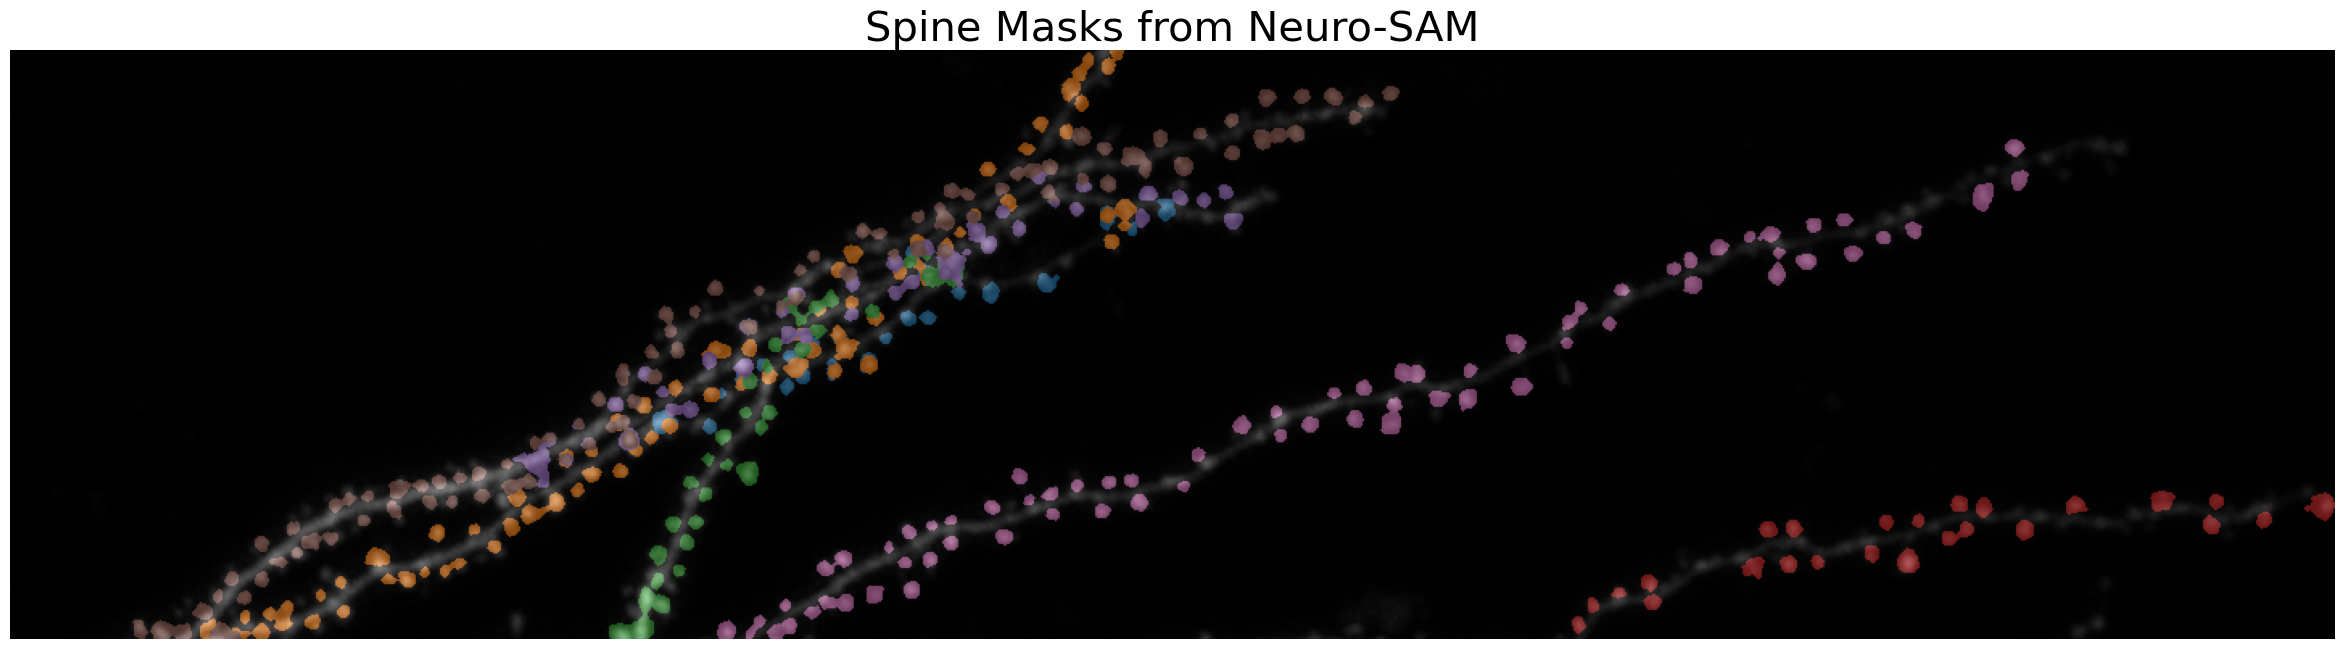
\includegraphics[width=0.95\textwidth]{figures/38_spine_seg_all.png}
\captionof{figure}{Overlay of spine segmentation masks predicted by Neuro-\gls{SAM} on the benchmark volume. Each spine instance is shown in a distinct color. The model localizes individual spines along dendritic shafts across diverse morphologies and densities. Scale: $0.94\,\mu\text{m}/\text{px}$}
\label{fig:spine_seg_all}
\end{center}

A representative visualization of spine segmentation masks generated by Neuro-\gls{SAM} is shown in \autoref{fig:spine_seg_all}, overlaid on the original benchmark stack. The output exhibits well-localized, evenly distributed spine predictions along the dendritic paths, capturing a wide range of spine shapes and sizes. To better illustrate prediction consistency, \autoref{fig:separate_spine_masks} presents slice-wise overlays of segmented spines on three traced paths from the volume. The predicted masks align closely with ground-truth spines, even in regions with densely clustered structures and low image contrast.

\begin{center}
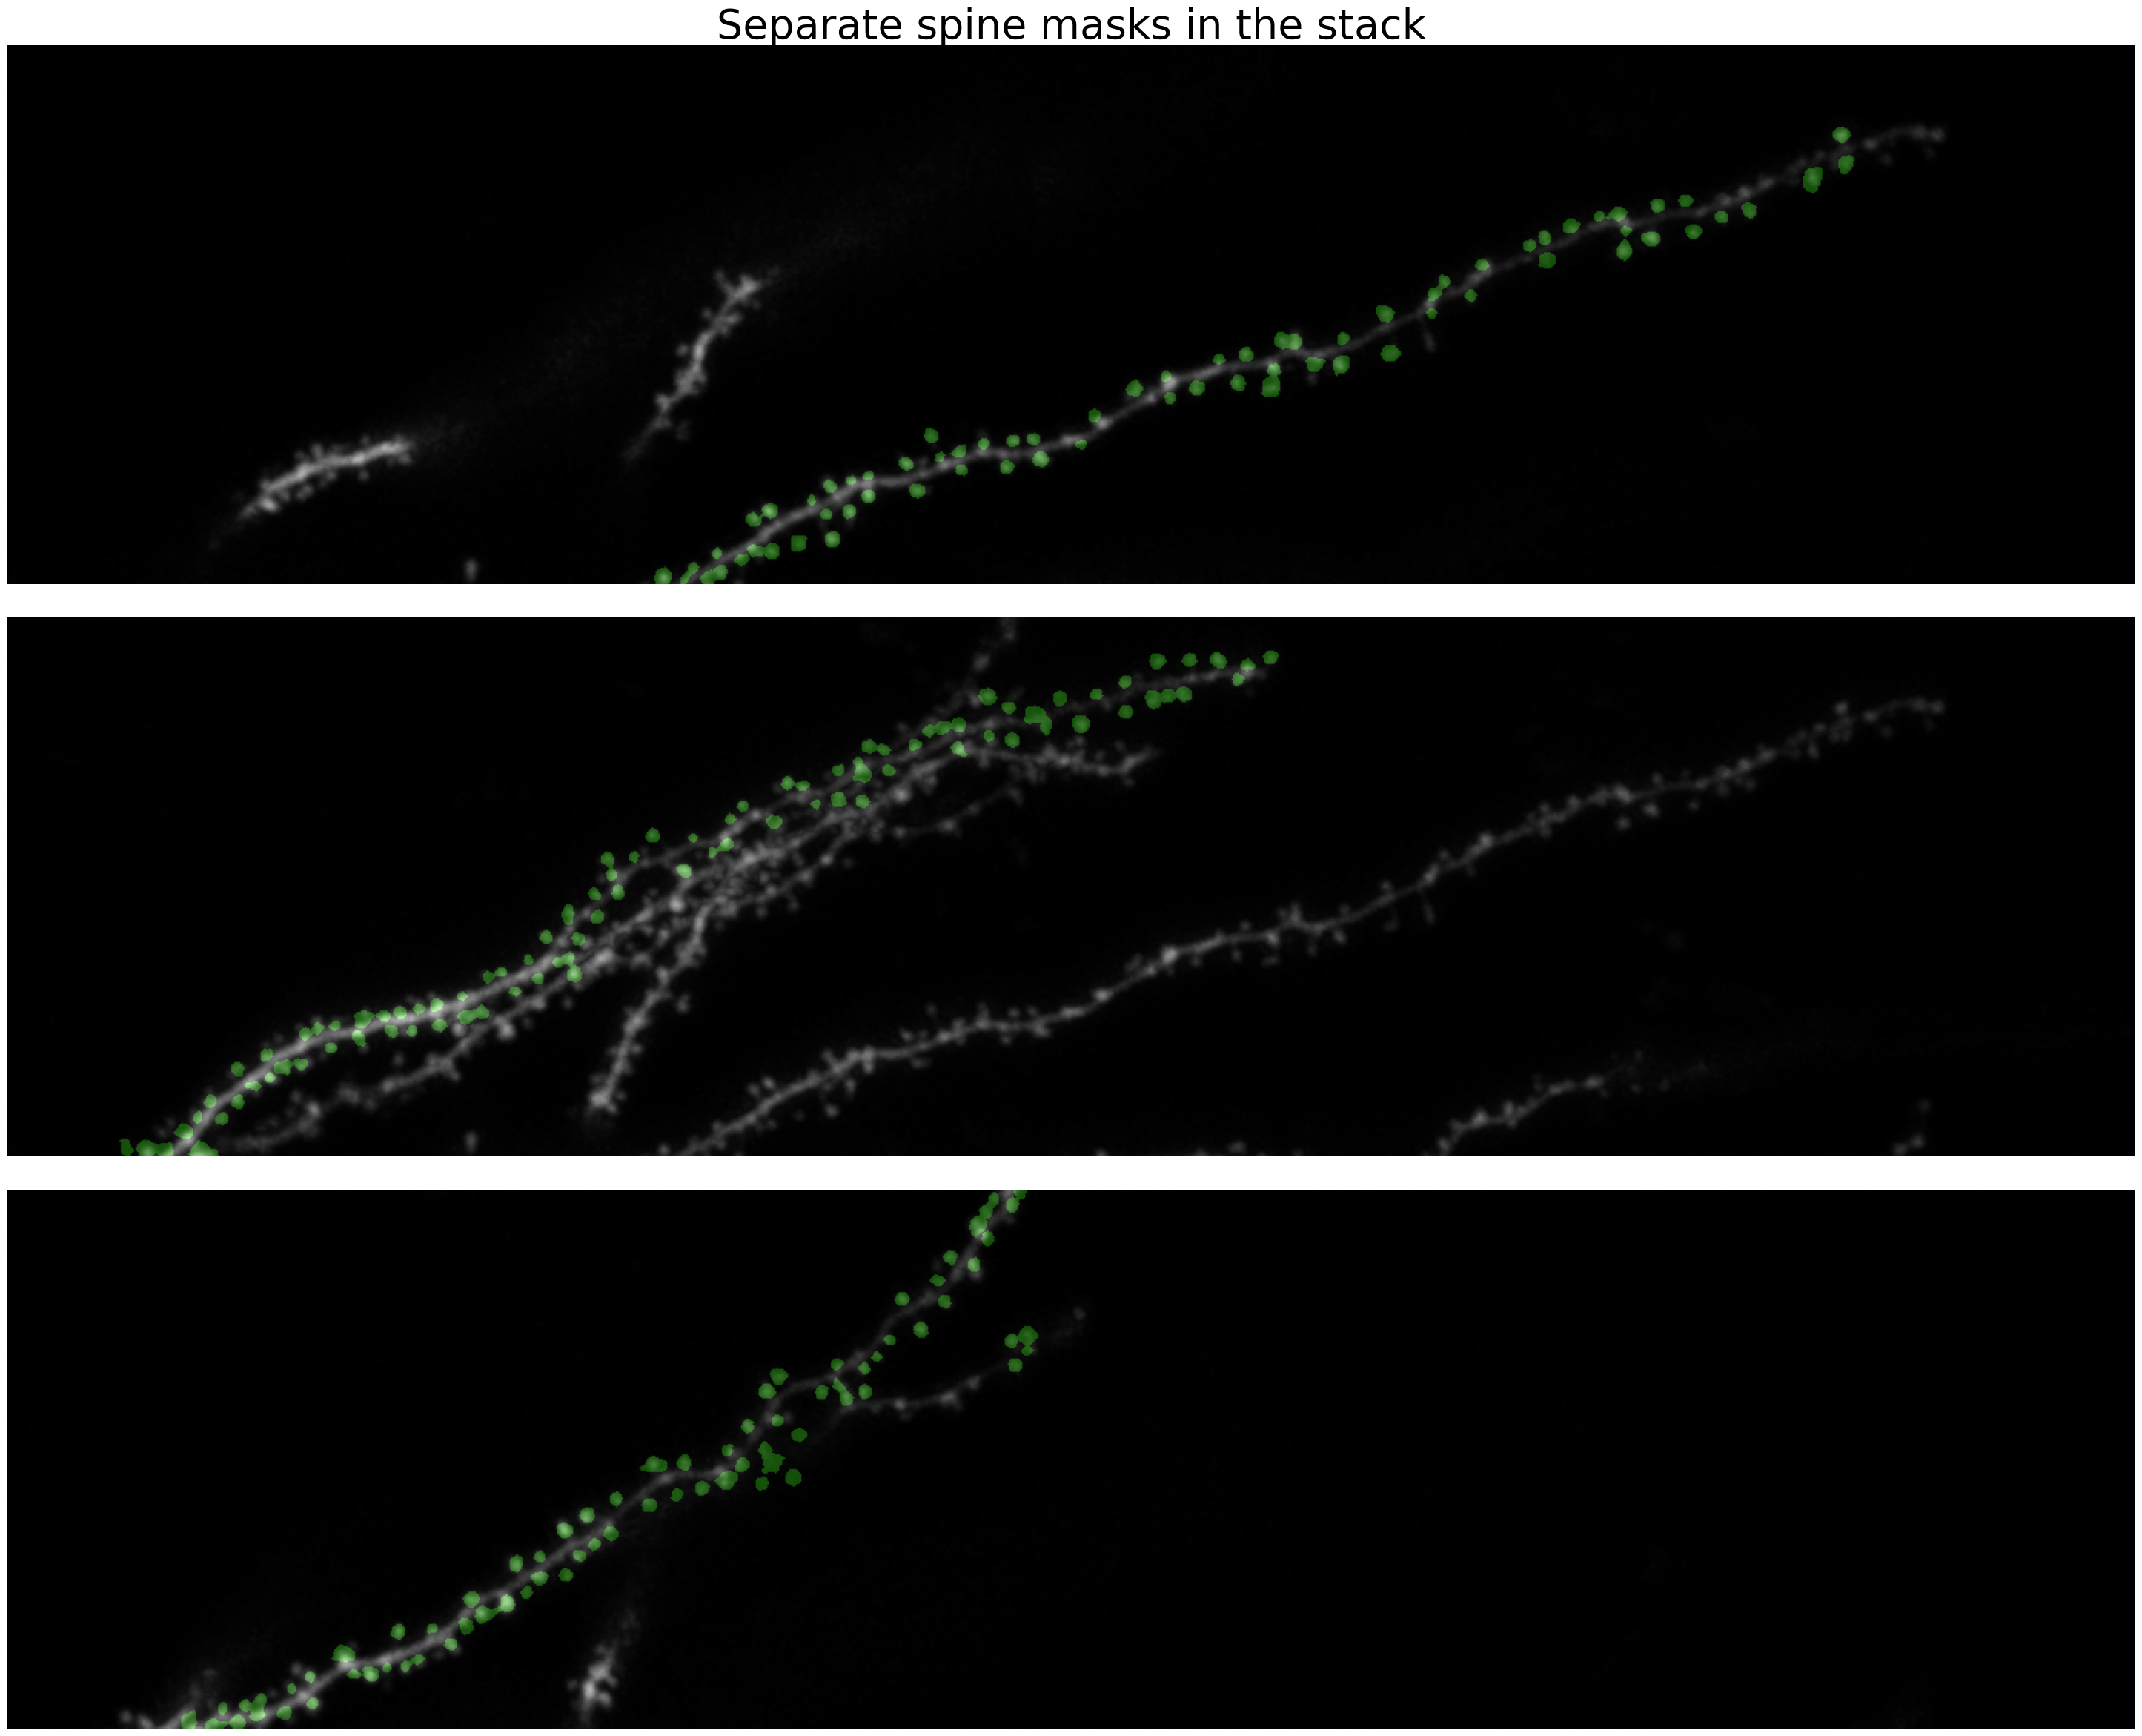
\includegraphics[width=0.8\textwidth]{figures/39_compare_frame_masks.png}
\captionof{figure}{Slice-wise visualization of predicted spines (green) by Neuro-\gls{SAM} on traced dendrites from the benchmark stack. Despite high spine density and low contrast regions, the model maintains spatial accuracy and continuity. Scale: $0.94\,\mu\text{m}/\text{px}$}
\label{fig:separate_spine_masks}
\end{center}

\begin{center}
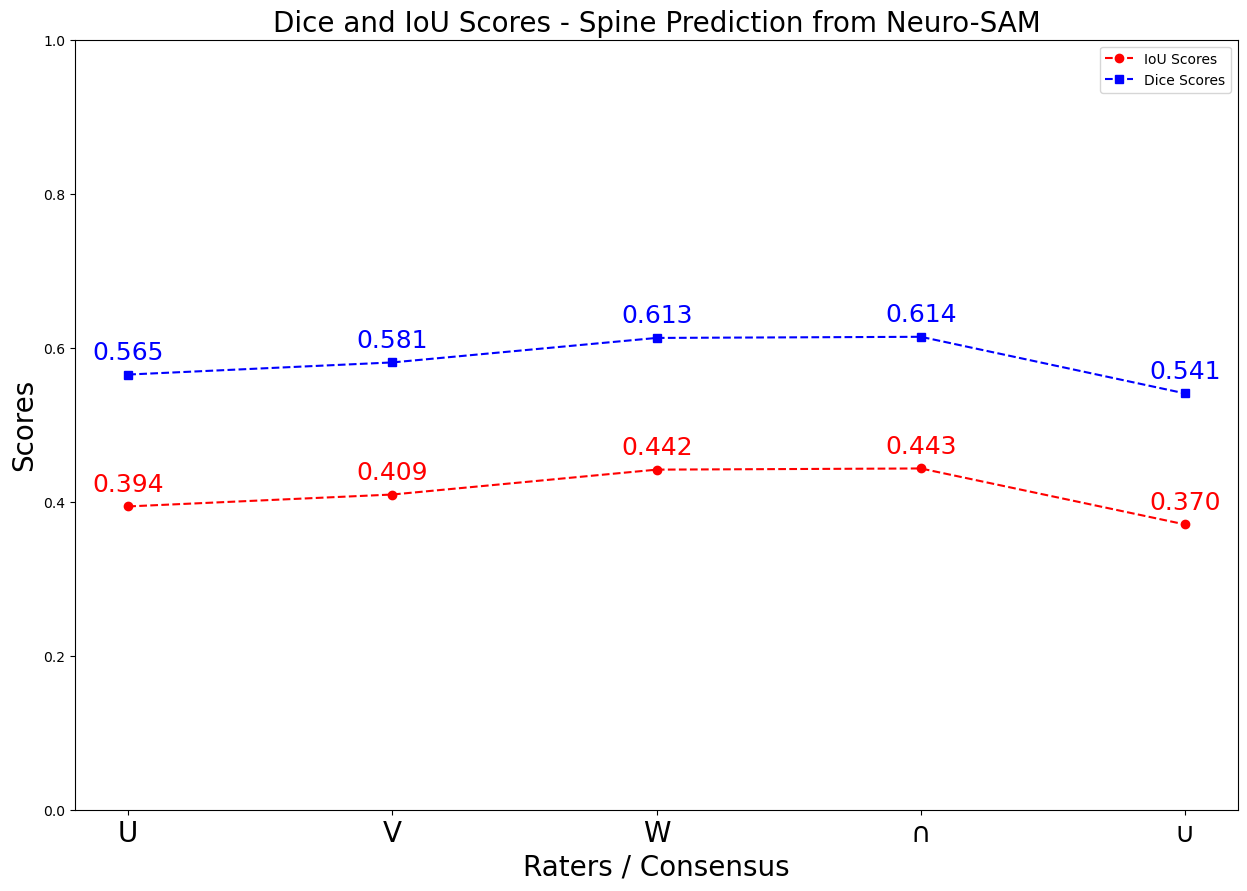
\includegraphics[width=0.8\textwidth]{figures/40_spine_seg_metrics.png}
\captionof{figure}{Quantitative evaluation of spine segmentation performance. Dice and \gls{IoU} scores from Neuro-\gls{SAM} predictions are computed against annotations from three human raters and the consensus. The model demonstrates consistent performance with minimal variability across raters.}
\label{fig:spine_seg_metrics}
\end{center}

Quantitative evaluation of spine segmentation performance is summarized in \autoref{fig:spine_seg_metrics}. Dice and \gls{IoU} scores across three raters and the unified consensus annotation highlight a strong performance by Neuro-\gls{SAM}, with average Dice scores ranging from 0.54 to 0.61 across raters. While performance is generally lower than dendrite segmentation due to the complexity and small size of spines, the consistency across raters indicates reliable model behavior.

\autoref{fig:spine_seg_comparison} compares spine segmentation outputs from \gls{DeepD3} and Neuro-\gls{SAM} against rater U. \gls{DeepD3} often shows slight over-segmentation and fragmented spines, whereas Neuro-\gls{SAM} yields more spatially compact and discrete spine masks. Finally, \autoref{fig:spine_seg_per_frame} shows per-frame performance comparisons, highlighting Neuro-\gls{SAM}’s capacity to maintain segmentation quality across diverse spatial regions and imaging conditions.


\begin{center}
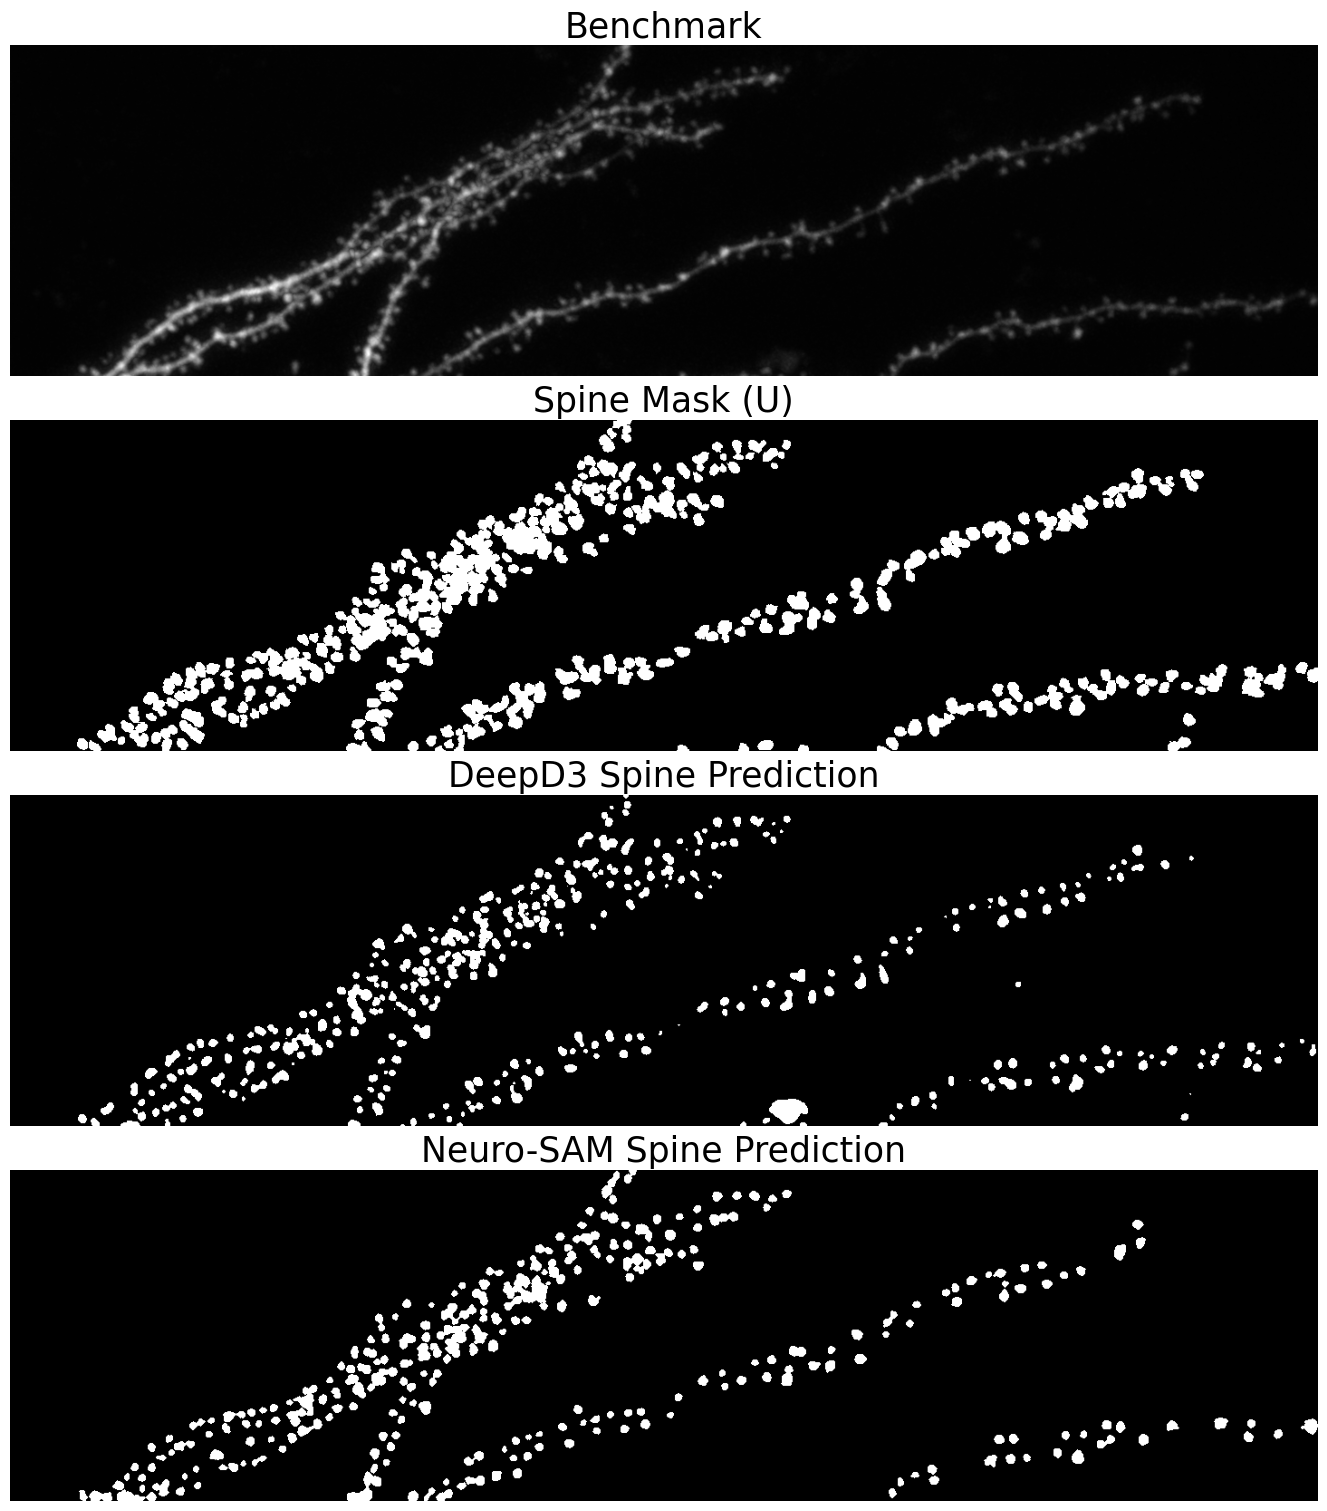
\includegraphics[width=0.9\textwidth]{figures/41_spine_seg_comparison.png}
\captionof{figure}{Comparative analysis of spine segmentation predictions from \gls{DeepD3} and Neuro-\gls{SAM}, with ground truth from rater U. Neuro-\gls{SAM} outputs exhibit better shape compactness and fewer false positives than \gls{DeepD3}. Scale: $0.94\,\mu\text{m}/\text{px}$}
\label{fig:spine_seg_comparison}
\end{center}


\begin{center}
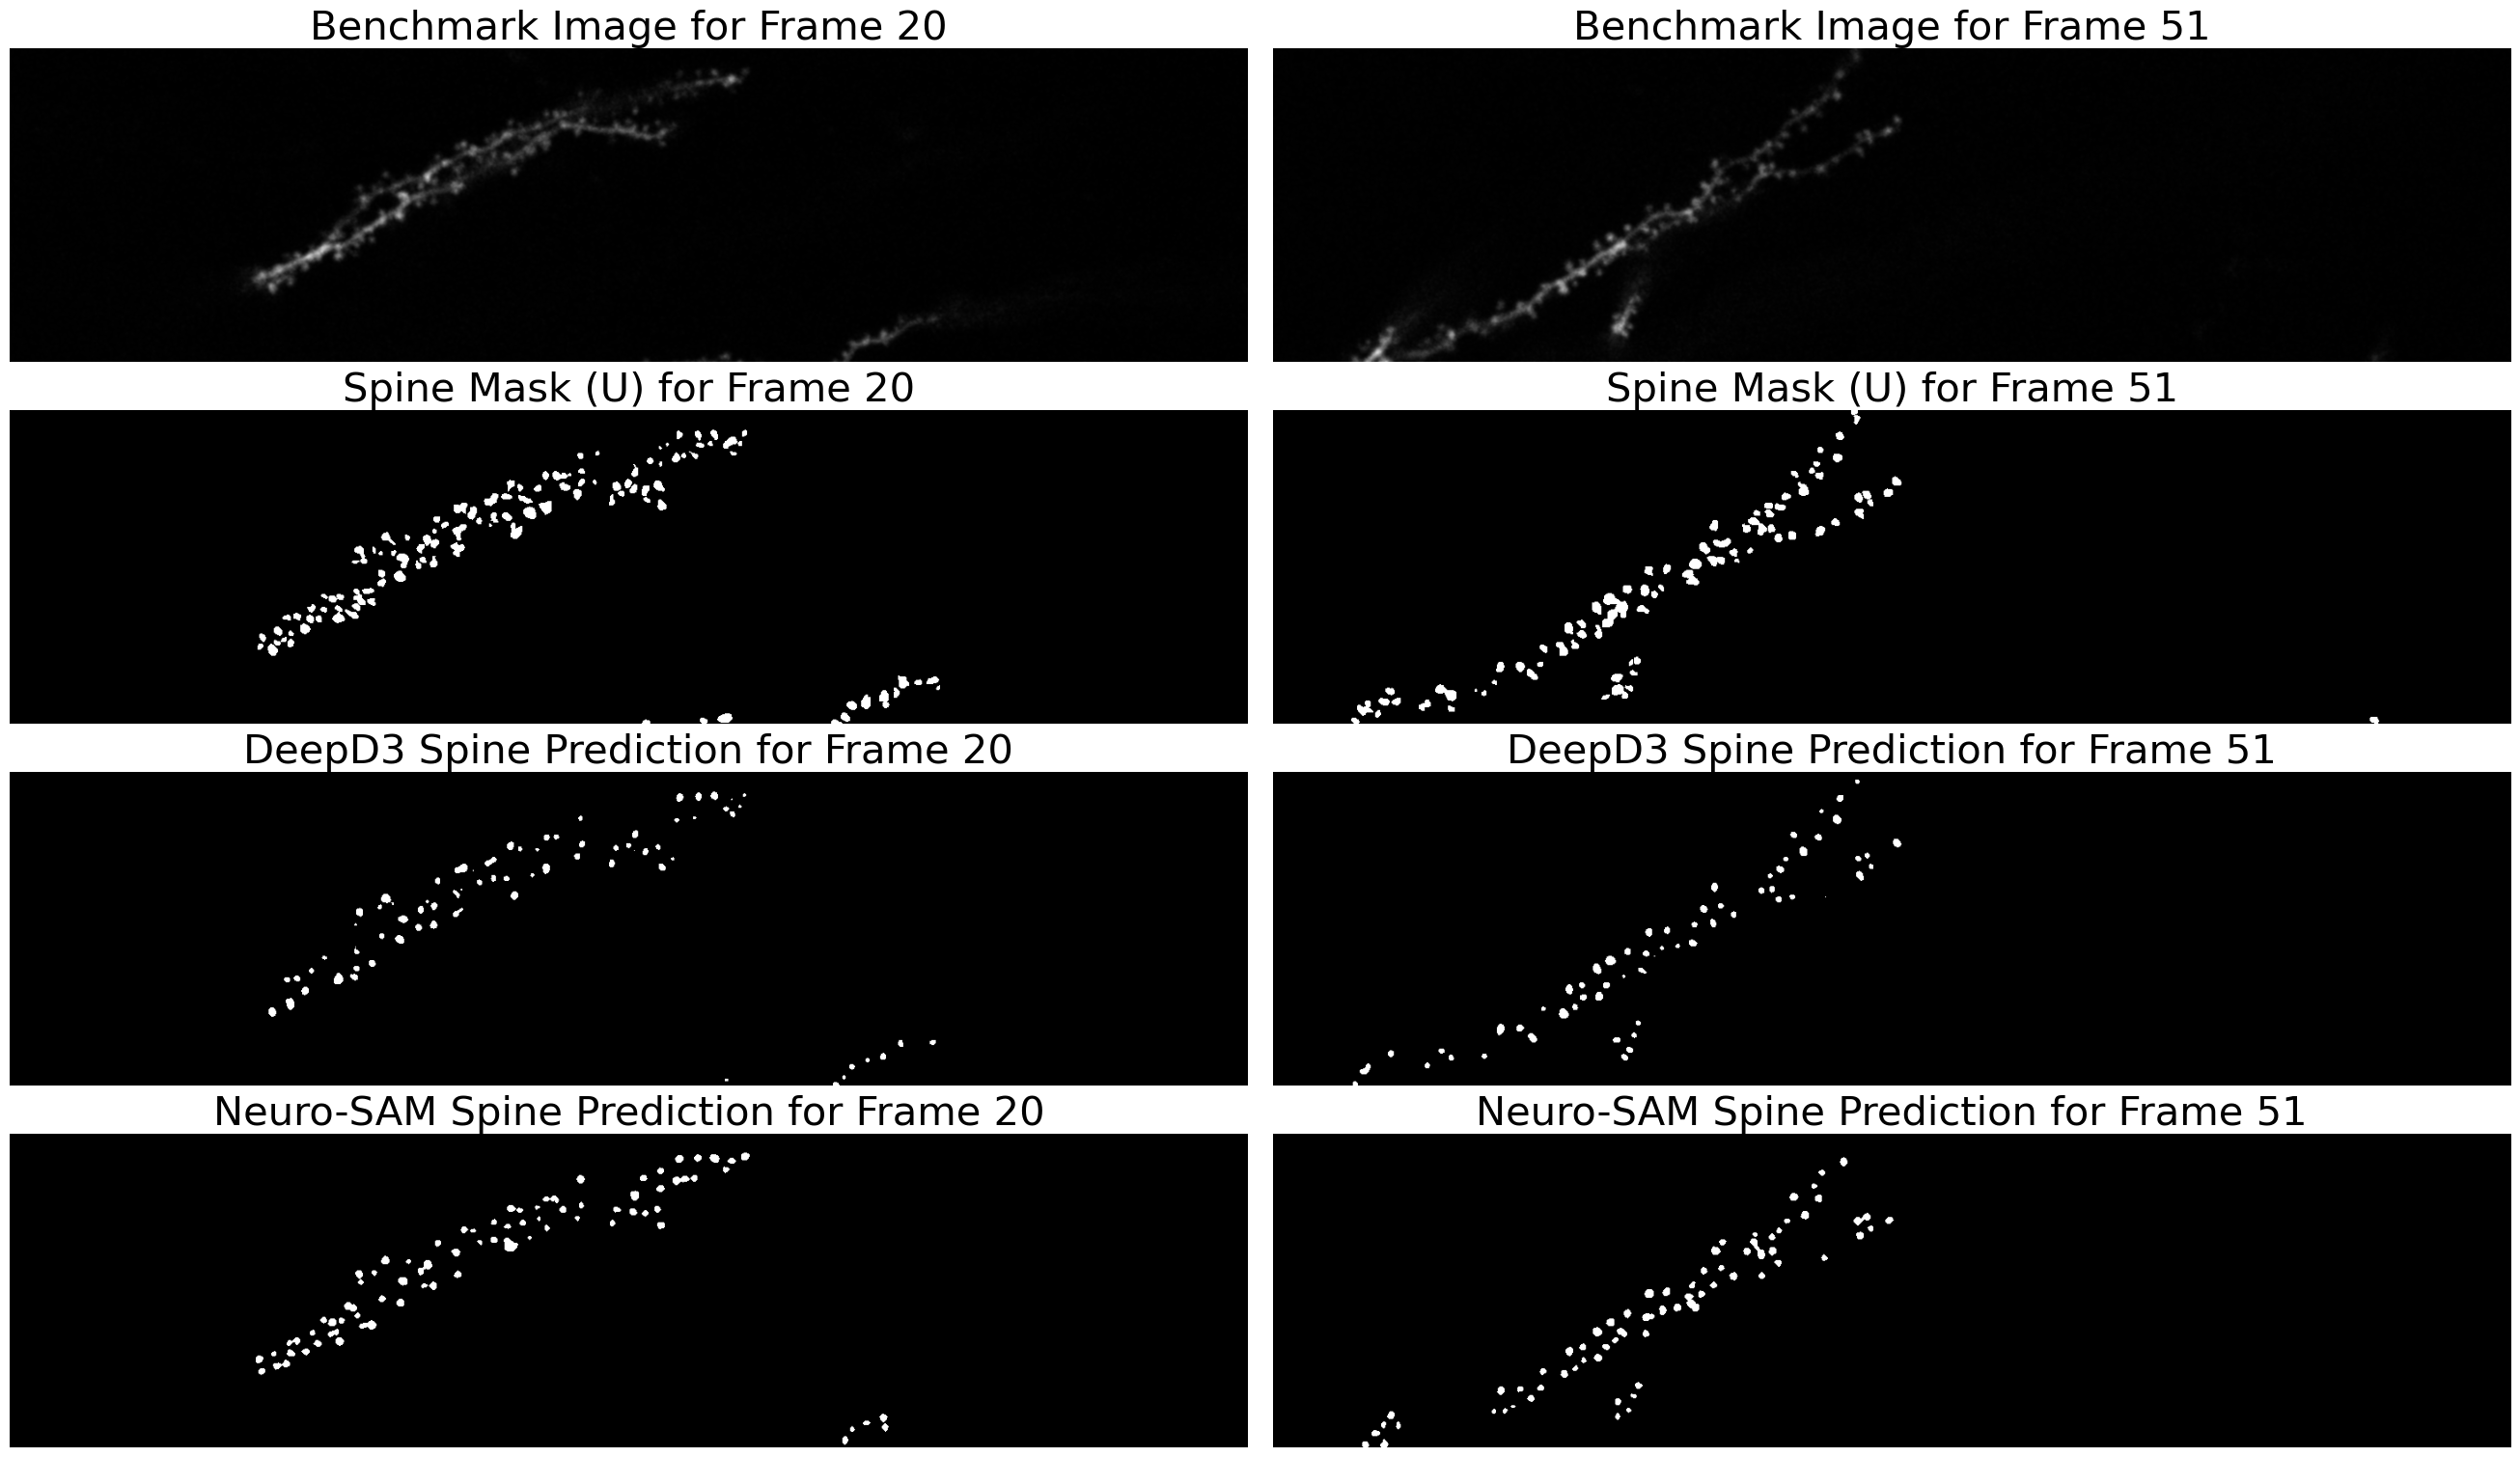
\includegraphics[width=0.95\textwidth]{figures/42_spine_seg_per_frame.png}
\captionof{figure}{Frame-wise segmentation results for spines on two different volumes. Top to bottom: raw benchmark image, ground truth annotation (rater U), \gls{DeepD3} prediction, and Neuro-\gls{SAM} prediction. Neuro-\gls{SAM} maintains more complete and consistent spine segmentation across frames. Scale: $0.94\,\mu\text{m}/\text{px}$}
\label{fig:spine_seg_per_frame}
\end{center}

\begin{center}
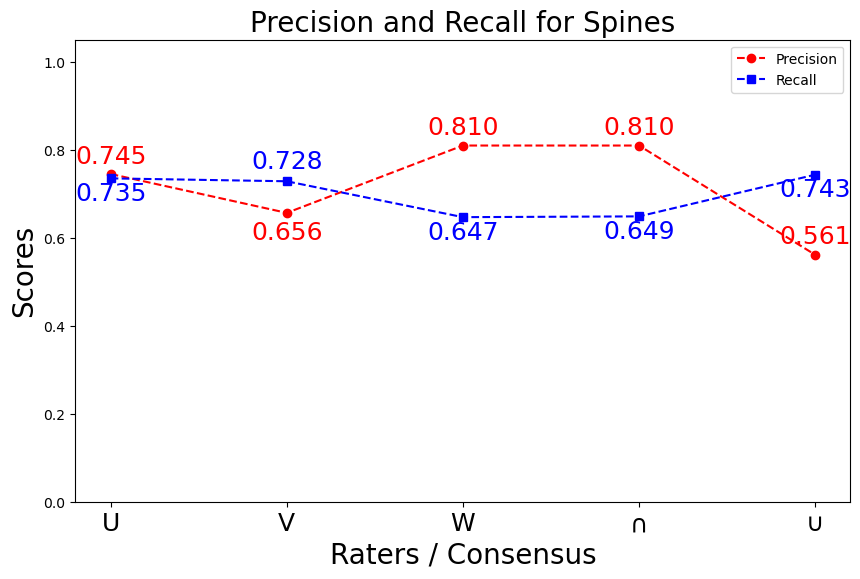
\includegraphics[width=0.8\textwidth]{figures/43_spine_precision_recall.png}
\captionof{figure}{Precision and recall scores for spine segmentation across individual raters and the consensus. Neuro-\gls{SAM} shows high precision with slightly lower recall, indicating conservative but accurate spine detection.}
\label{fig:spine_precision_recall}
\end{center}


In addition to Dice and \gls{IoU}, we analyzed the precision and recall of Neuro-\gls{SAM}’s spine predictions across all raters and the consensus (\autoref{fig:spine_precision_recall}). Neuro-\gls{SAM} exhibits high precision, particularly against raters W and $\cap$, indicating strong specificity with minimal false positives. However, recall is moderately lower, suggesting that a few spines may be missed, especially in densely clustered regions. This trade-off highlights the bias of Neuro-\gls{SAM} towards conservative segmentation, which is often desirable in scenarios where false positives can impede downstream analyses.

\begin{center}
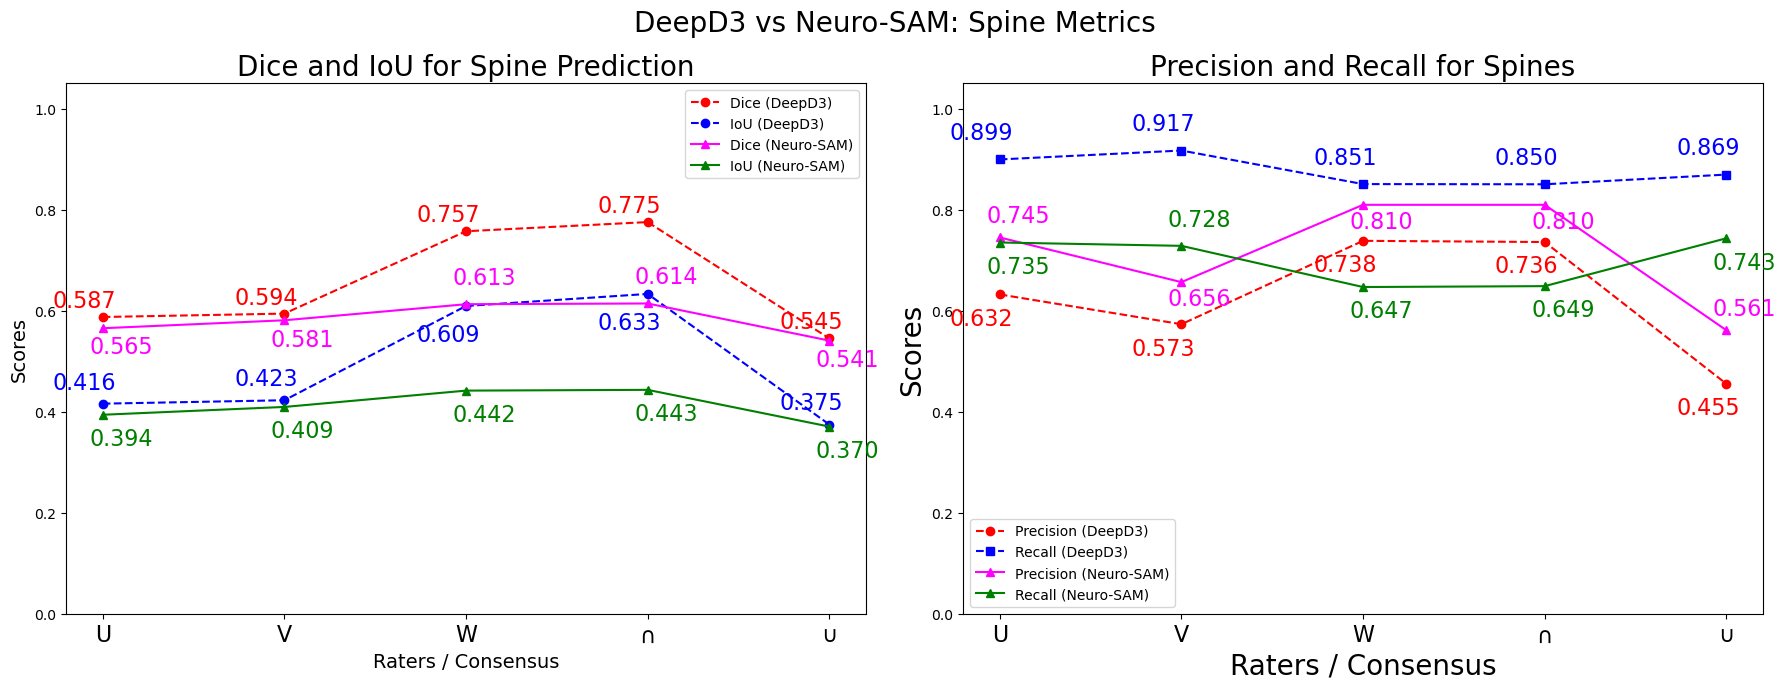
\includegraphics[width=0.98\textwidth]{figures/44_deepd3_neurosam_comparison.png}
\captionof{figure}{Comparison of \gls{DeepD3} and Neuro-\gls{SAM} on Spine Segmentation Metrics. Neuro-\gls{SAM} achieves higher precision with balanced Dice and \gls{IoU} scores, while \gls{DeepD3} demonstrates higher recall, indicating a tendency toward over-segmentation.}
\label{fig:deepd3_neurosam_comparison}
\end{center}

To further contextualize the performance of Neuro-\gls{SAM}, we conducted a head-to-head comparison with \gls{DeepD3} across Dice, \gls{IoU}, Precision, and Recall metrics. As shown in \autoref{fig:deepd3_neurosam_comparison}, \gls{DeepD3} exhibits higher recall values across all raters, suggesting that it captures more spines. In contrast, Neuro-\gls{SAM} maintains a more balanced trade-off, showing consistently higher precision while preserving reasonable recall. This conservative segmentation strategy, informed by dendrite-aware prompting and high-resolution fine-tuning, results in fewer false detections and better anatomical alignment. In addition, the Dice and \gls{IoU} scores remain comparable between both methods, underscoring the robustness and efficiency of Neuro-\gls{SAM} in generating high-quality spine masks even under noisy or ambiguous imaging conditions.

Together, these results demonstrate that Neuro-\gls{SAM} effectively extends its path-based spatial awareness to high-precision spine segmentation. While inter-rater variability and dense spatial arrangements present inherent challenges, Neuro-\gls{SAM} maintains coherent predictions, underscoring its potential as a scalable and annotation-efficient tool for fine-grained structural analysis in neuroscience.

\subsection{Generalization across other datasets}
To evaluate the robustness and adaptability of Neuro-\gls{SAM} beyond the benchmark dataset, we tested its performance on additional dendritic imaging datasets with varying signal-to-noise ratios, staining techniques, and imaging conditions. These datasets were never seen during training and were selected to challenge the model’s ability to generalize to unseen morphological patterns and contrast variations. In all cases, the full Neuro-\gls{SAM} pipeline was applied without re-training or fine-tuning. The goal of this evaluation is to assess whether our path-conditioned prompting and modular design generalize well to diverse settings while maintaining structural fidelity.

\begin{center}
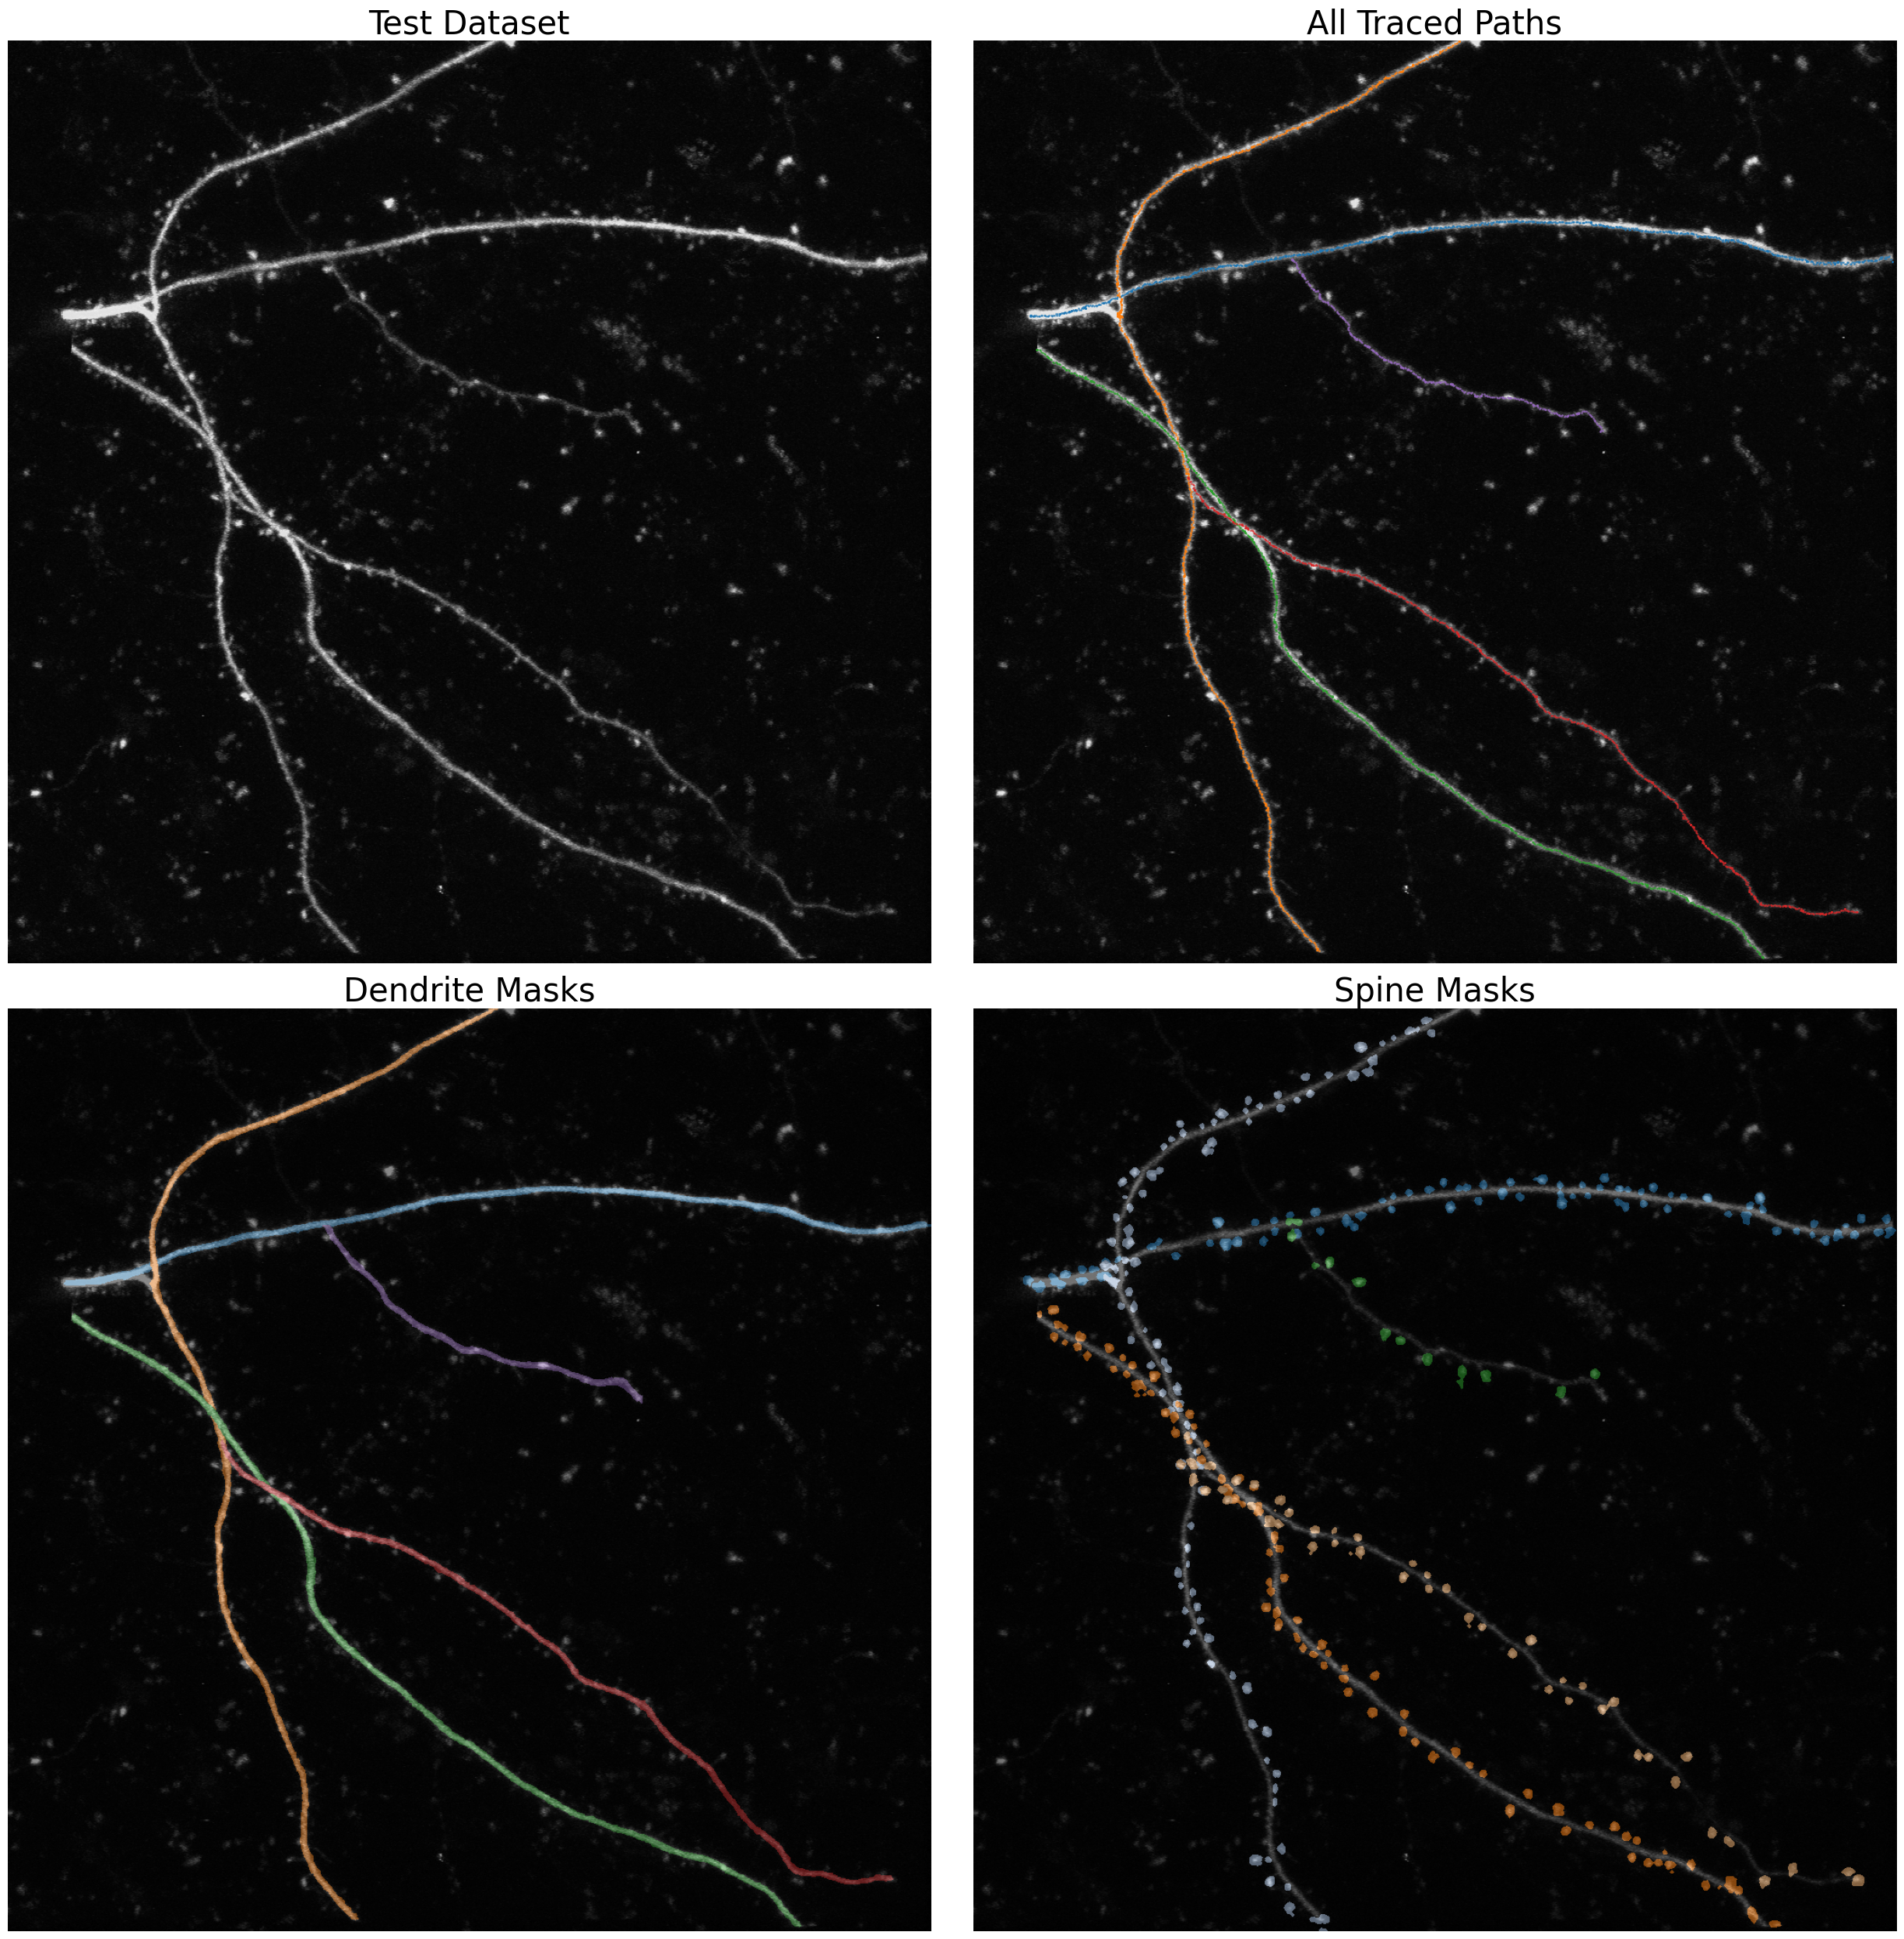
\includegraphics[width=0.95\textwidth]{figures/46_generalization_stack1.png}
\captionof{figure}{Robust results of Neuro-\gls{SAM}. The model successfully traces dendritic paths (top-right), segments dendrite shafts (bottom-left), and identifies individual spines (bottom-right) despite visual differences from the benchmark dataset. Scale: $1\,\mu\text{m}/\text{px}$}
\label{fig:generalization_stack1}
\end{center}

As illustrated in \autoref{fig:generalization_stack1}, Neuro-\gls{SAM} pipeline was also applied on this dataset. The model was able to robustly trace complex dendritic structures and generate precise, continuous masks even in morphologically and visually distinct regions. In particular, spine segmentation also remained consistent, with clear spatial alignment along the traced dendrites. These results highlight the adaptability of the pipeline to new domains, underscoring its utility in low-annotation or cross-laboratory settings.

\begin{center}
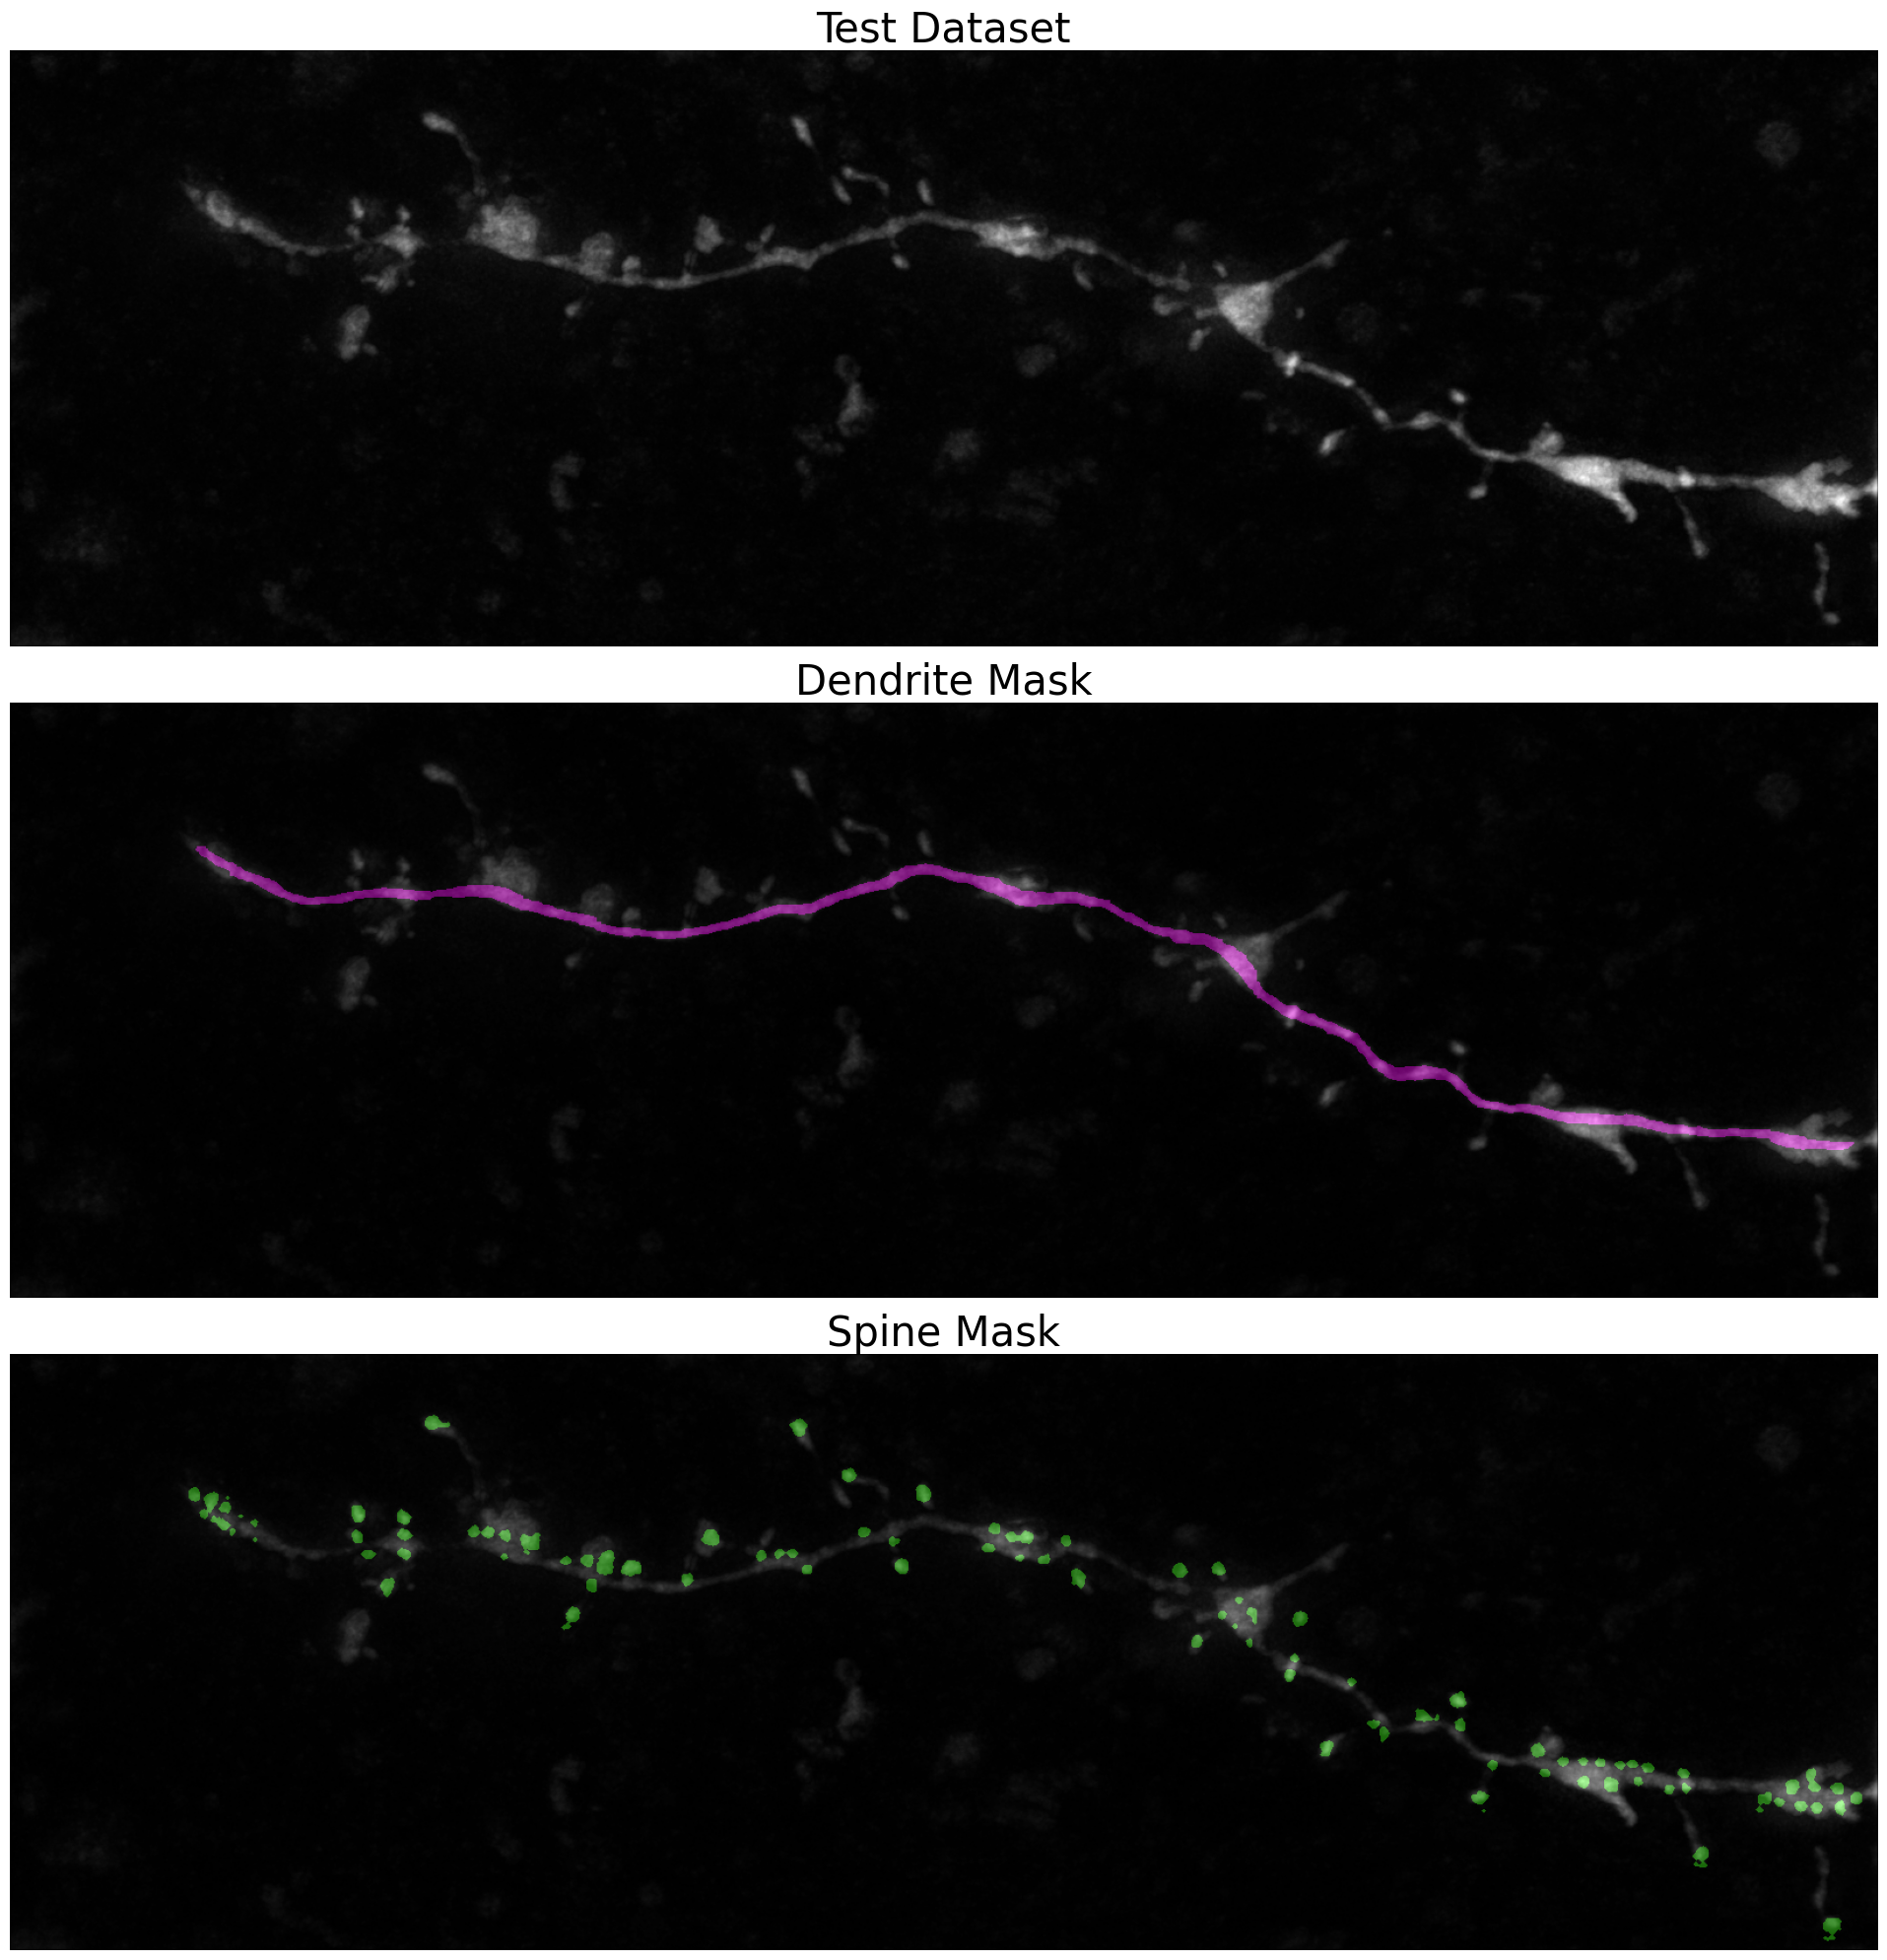
\includegraphics[width=0.8\textwidth]{figures/47_generalization_stack2.png}
\captionof{figure}{Generalization performance of Neuro-\gls{SAM} on a morphologically diverse dataset. Despite noise and complex spine shapes, the model accurately segments the dendrite shaft and detects the majority of spines along its path Scale: $1\,\mu\text{m}/\text{px}$}
\label{fig:generalization_stack2}
\end{center}

In a second generalization test, Neuro-\gls{SAM} was evaluated on a dataset with highly variable spine morphology and lower signal-to-noise ratio. As shown in \autoref{fig:generalization_stack2}, the dendrite was successfully traced and segmented with strong continuity, even across subtle changes in thickness and contrast. Spine segmentation was largely successful, capturing most spines along the shaft. However, in denser regions or where the spines were faint or elongated, the model occasionally missed or under-segmented structures. These results highlight that while Neuro-\gls{SAM} generalizes robustly, performance can be further strengthened by incorporating more morphologically diverse training samples or refining prompt adaptation strategies for challenging conditions.

\begin{center}  
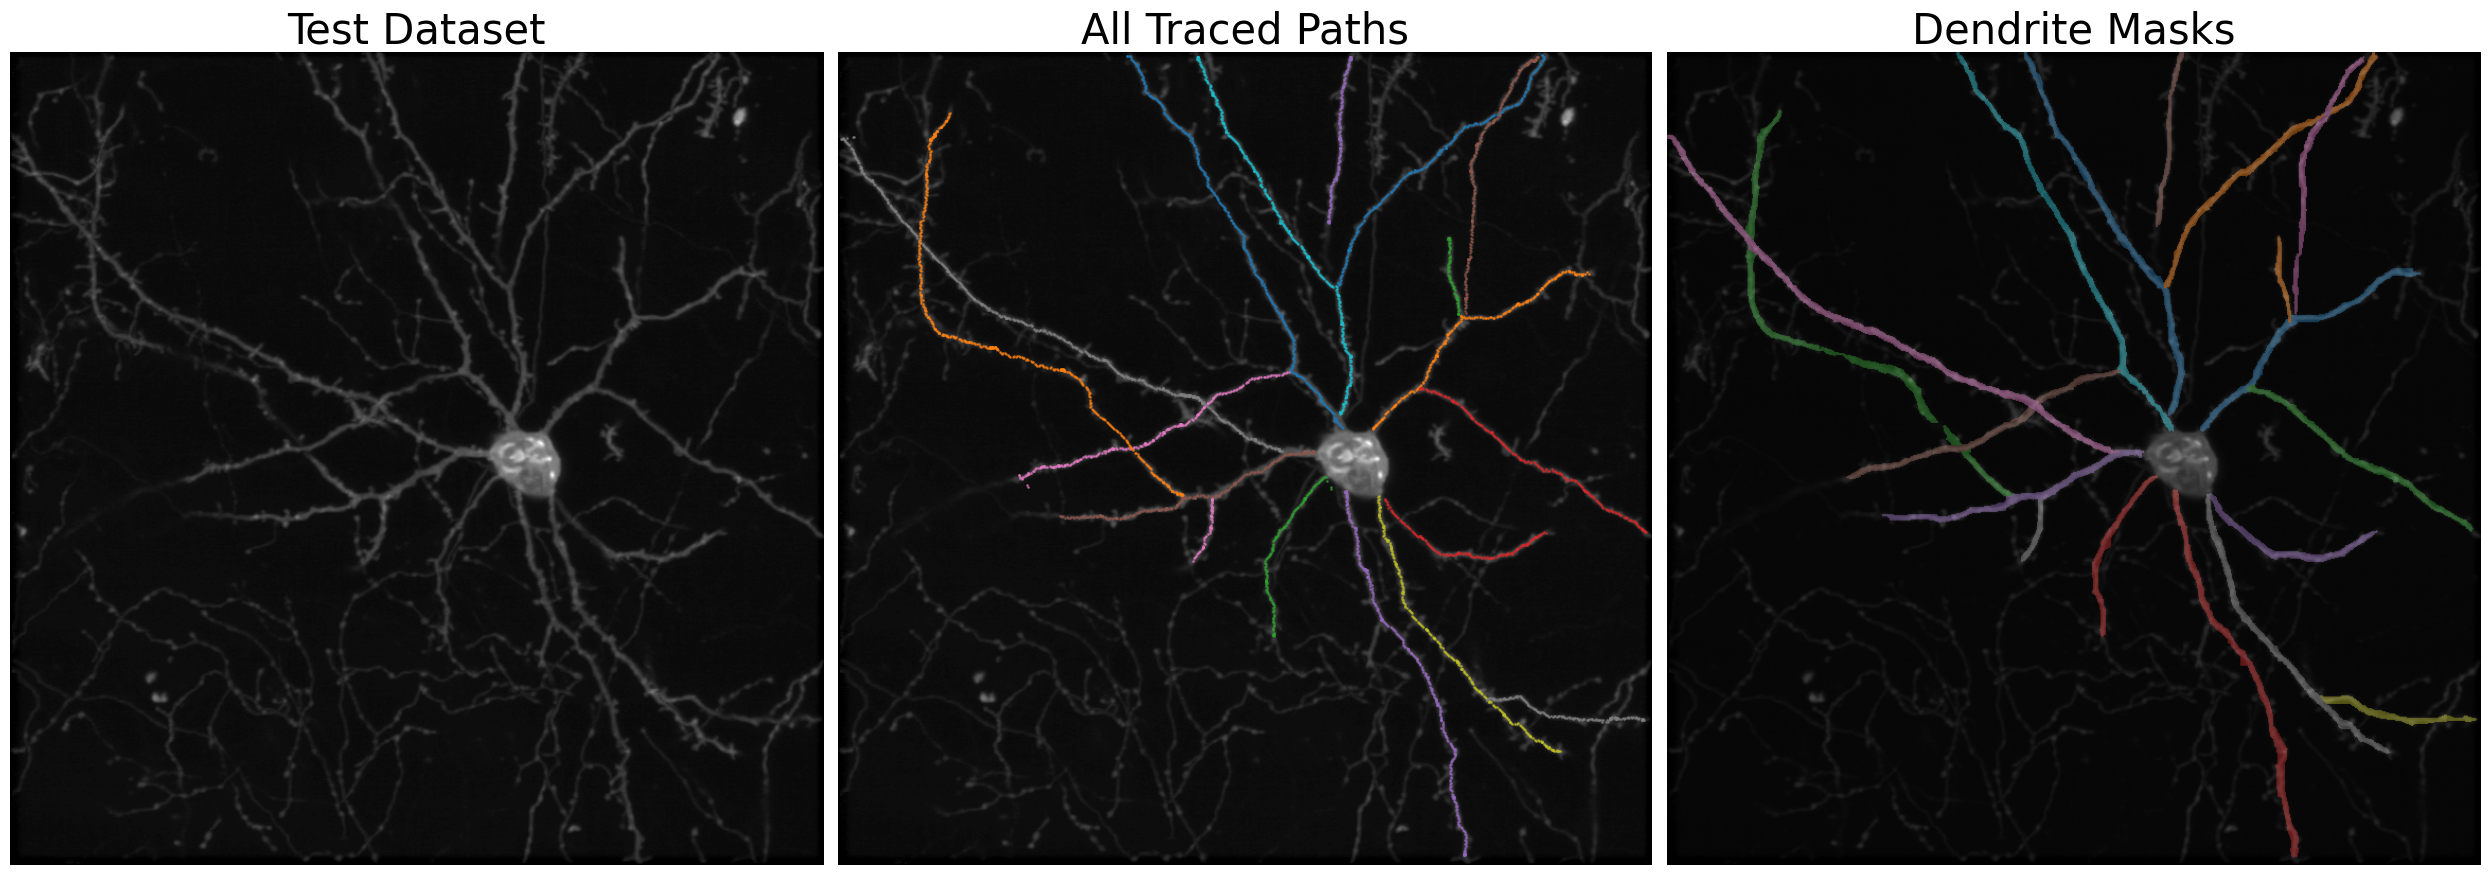
\includegraphics[width=0.98\textwidth]{figures/48_generalization_stack3.png}  
\captionof{figure}{Generalization of Neuro-\gls{SAM} on a full-neuron dataset. Left: raw test dataset. Middle: traced dendritic paths. Right: dendrite segmentation masks. Spine detection was not performed due to very few visible spines. Scale: $1\,\mu\text{m}/\text{px}$}  
\label{fig:generalization_stack3}  
\end{center}  

As a final generalization test, Neuro-\gls{SAM} was applied to a dataset containing a complete neuron with extensive arborization (\autoref{fig:generalization_stack3}). Despite the increased structural complexity and large number of intersecting branches, the model reliably traced all dendritic paths from the soma and generated coherent segmentation masks for each shaft. Since this dataset contained very few visible spines, spine detection and segmentation were not performed. Nevertheless, the results confirm that Neuro-\gls{SAM} can maintain structural fidelity at whole-cell scale, effectively capturing both global morphology and fine local detail. This experiment underscores the framework’s adaptability for large-scale reconstructions, positioning it as a practical tool for comprehensive neuroanatomical mapping.

